
\documentclass[a4paper]{article}
\usepackage[utf8]{inputenc}
\usepackage[italian]{babel}


%\renewcommand{\thesection}{\arabic{section}} % to avoid chapters
\usepackage{geometry}
\usepackage{graphicx}
\usepackage{colortbl}
\let\footruleskip\undefined
\usepackage{fancyhdr}
\usepackage{lastpage}
\usepackage{verbatim}
\usepackage[shortlabels]{enumitem}
\pagestyle{fancyplain}
\usepackage{amsmath}
\usepackage{subfig}
\usepackage[dvipsnames]{xcolor}
\usepackage[export]{adjustbox}
\fancyhead[l]{\leftmark}
\fancyhead[r]{gennaio, 2020}
\setlength\parindent{10pt}
\setlength\parskip{5pt}
\usepackage{amsmath} % must be included for cleveref to work
\usepackage[hidelinks]{hyperref}
\usepackage[nameinlink]{cleveref}
\graphicspath{{./images/}}
\usepackage{listings}
\usepackage{xcolor}
\usepackage[space]{grffile}
\usepackage{caption}
\usepackage{dirtytalk}
\usepackage{blindtext}

\DeclareCaptionType{equ}[][]

\definecolor{codegreen}{rgb}{0,0.6,0}
\definecolor{codegray}{rgb}{0.5,0.5,0.5}
\definecolor{codepurple}{rgb}{0.58,0,0.82}
\definecolor{backcolour}{rgb}{0.95,0.95,0.92}
\definecolor{backcolourbash}{rgb}{0.65,0.65,0.8}
\definecolor{codegreenbash}{rgb}{0.9,0.9,0.9}

\lstdefinestyle{mystyle}{
	backgroundcolor=\color{backcolour},   
	commentstyle=\color{codegreen},
	keywordstyle=\color{magenta},
	numberstyle=\tiny\color{codegray},
	stringstyle=\color{codepurple},
	basicstyle=\ttfamily\footnotesize,
	breakatwhitespace=false,         
	breaklines=true,                 
	captionpos=b,                    
	keepspaces=true,                 
	numbers=left,                    
	numbersep=5pt,                  
	showspaces=false,                
	showstringspaces=false,
	showtabs=false,                  
	tabsize=2
}

\lstdefinestyle{customBash}{
	backgroundcolor=\color{backcolourbash},   
	commentstyle=\color{codegreenbash},
	keywordstyle=\color{magenta},
	numberstyle=\tiny\color{codegray},
	stringstyle=\color{codepurple},
	basicstyle=\ttfamily\footnotesize,
	breakatwhitespace=false,         
	breaklines=true,                 
	captionpos=b,                    
	keepspaces=true,                 
	numbers=left,                    
	numbersep=5pt,                  
	showspaces=false,                
	showstringspaces=false,
	showtabs=false,                  
	tabsize=2
}

\definecolor{lbcolor}{rgb}{0.9,0.2,0.2} 
 


\lstset{style=mystyle}

\usepackage{array}
\newcolumntype{L}[1]{>{\raggedright\let\newline\\\arraybackslash\hspace{0pt}}m{#1}}
\renewcommand{\arraystretch}{2} % This command might break stuff, but makes tabulars much more readable

% Used to include TODO's in the document
\usepackage[colorinlistoftodos]{todonotes}

\usepackage{caption}

\usepackage{titlesec}
\titleformat{\chapter}[hang] 
{\normalfont\huge\bfseries}{\thechapter}{1em}{}

% \titlespacing{command}{left spacing}{before spacing}{after spacing}[right]
% spacing: how to read {12pt plus 4pt minus 2pt}
%           12pt is what we would like the spacing to be
%           plus 4pt means that TeX can stretch it by at most 4pt
%           minus 2pt means that TeX can shrink it by at most 2pt
%       This is one example of the concept of, 'glue', in TeX
\titlespacing\chapter{0pt}{8pt plus 4pt minus 2pt}{8pt plus 2pt minus 2pt}

\usepackage{tabularx}               % Enables tabluarx environment
\usepackage{booktabs}               % Lines for tables
\usepackage{float}
\restylefloat{table}

%glossaries
\usepackage[automake]{glossaries}
\setacronymstyle{long-short}
\makeglossaries
\glstoctrue
\setglossarystyle{altlist}

\newcommand{\newabbrentry}[4]{%
	\newglossaryentry{#1}{
		name={ \makefirstuc{#3} (#2)},
		first={#3 (#2)},
		description={#4},
		text={#2}
	}
}

% task description table counters
\newcounter{i}
\newcounter{j}

\usepackage[backend=biber,style=numeric,sorting=none]{biblatex}
\addbibresource{bibliografia.bib}
\usepackage{wrapfig}


\begin{document}
	
\begin{titlepage}
    \begin{center}
		\vspace*{\fill}

		\vspace{2cm}
        \Huge\textbf{Titolo}\\
        
        \vspace{4cm}
        \vspace{1.5cm}
        \Large{Cavagna Giorgio}\\
        \vspace{0.5cm}
        %\Large{Group 7}\\
        \vspace{0.5cm}
        \large{15 Gennaio, 2020}
        \vspace*{\fill}
    \end{center}  
\end{titlepage}



	%\printglossary[type=\acronymtype, title=Abbreviations]
	
	\setcounter{tocdepth}{3}
	%\tableofcontents
	
	
	% Chapters
	\newpage
	\tableofcontents
	\newpage
	\section{Introduzione}
Ho deciso di presentare la proposta per la realizzazione di un chiosco in riva ad un lago.
L'idea del progetto è nata parlando con la mia professoressa, visto che ad entrambi piace il lago di Endine.
Notando  la scarsità di edifici adibiti a bar, sul percorso pedonale che costeggia il lago, ho immaginato e progettato una struttura che avesse questo scopo ma che si integrasse con l’ambiente circostante .

Ho così individuato una struttura esistente in disuso per potere usufruire dell'ingombro e ottenere con maggiore facilità i permessi dal comune ed enti predisposti. 


Nella tesi ho descritto l’ambiente dove sarà collocato il chiosco ed ho sviluppato il progetto partendo da una struttura disegnata dall'architetto Natasha Kwok che mi è particolarmente piaciuta per le sue forme.
In funzione della struttura esterna ho progettato  la zona bar e la disposizione dei vari moduli,facendo attenzione ad applicare le regole ergonomiche.

L'area circostante presenta delle criticità per le quali ho pensato a delle soluzioni applicabili per rendere il posto più confortevole.

	\newpage
	\section{Inquadramento territoriale}

Il lago di Endine (\cref{fig:mappa})si trova nell'alta Val Cavallina, dove si è formato nell'epoca quaternaria in seguito ai movimenti di escavazione dovuti al movimento delle masse glaciali. Il lago è classificato come lago glaciale vallivo. Confrontato con altri laghi di origine glaciale, è caratterizzato da una profondità media relativamente bassa.
La scarsa profondità ha giocato un ruolo fondamentale nei processi di degrado ambientale e successivo recupero, che ha interessato il lago negli ultimi 50 anni. 

Il bacino lacustre presenta la conformazione tipica dei laghi di origine glaciale: ha una forma allungata secondo l’andamento della valle che occupa la parte centrale, donandole caratteristiche peculiari tra cui una variegata flora spontanea. 
Con una forma allungata, lungo l’asse nord-est, sud-ovest. Il lago è situato a 340 metri di altitudine ed è alimentato da numerosi torrenti che scendono dai monti circostanti e ha un unico emissario, il Cherio, che scorre poi nella pianura per poi confluire nell'Oglio.

Sulle sponde del lago si affacciano quattro comuni: Spinone, Ranzanico, Endine Gaiano e Bianzano.

\begin{figure}[H]
	\centering
	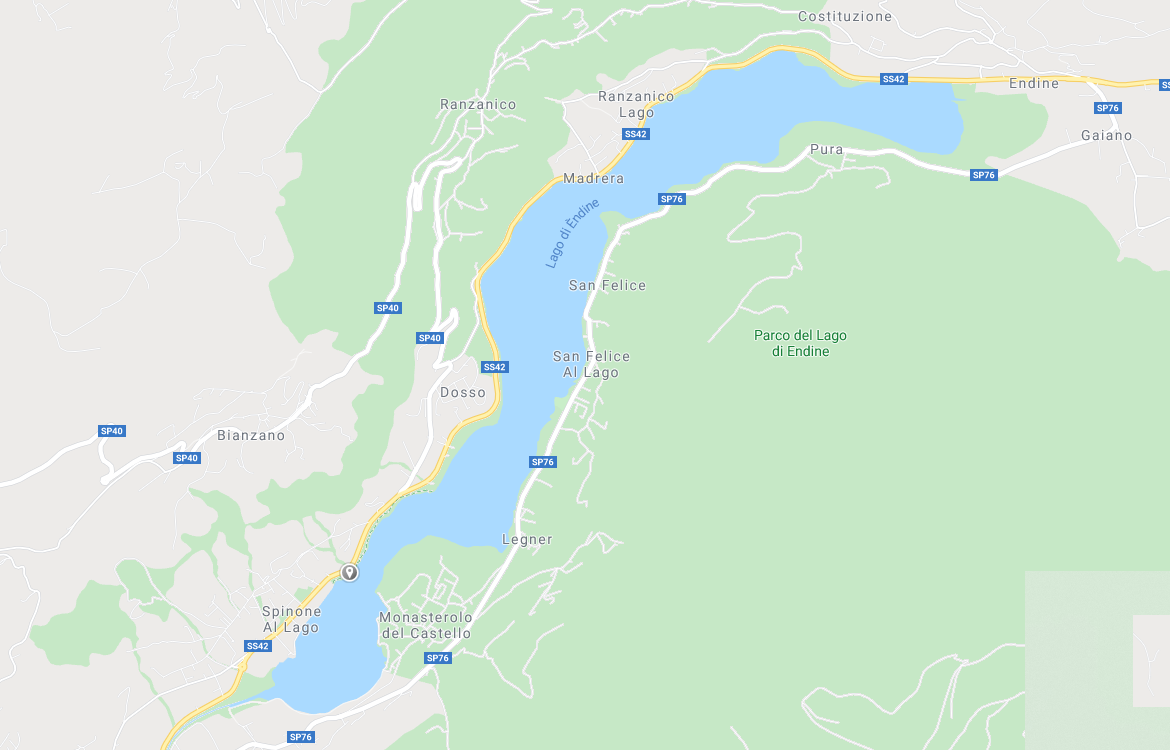
\includegraphics[width=0.6\textwidth]{image12}
	\caption{Mappa}
	\label{fig:mappa}
\end{figure}

Il lago, incassato nella stretta valle tra alti rilievi, ha conservato pressoché intatto l'ambiente naturale; classificato in un primo tempo come zona di rilevante interesse ambientale dalla Regione Lombardia; successivamente come parco e come tale soggetto a tutela. Le rive alternano fitti canneti, che sono luogo di riproduzione della ricca fauna ittica e rifugio per la fauna avicola, a piccole spiagge molto frequentate nei fine settimana da turisti che vi possono consumare la colazione al sacco in aree appositamente attrezzate; ma anche vi si può praticare  sport d'acqua, tra cui: vela, windsurf, canoa, canottaggio ed infine la pesca.

\begin{figure}[H]
	\captionsetup[subfloat]{farskip=2pt,captionskip=8pt}
	\centering
	\subfloat[M. Girone]{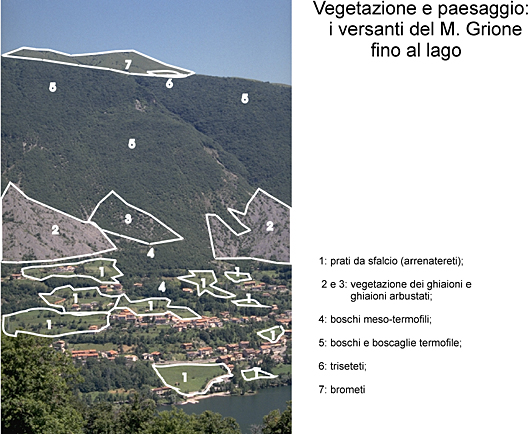
\includegraphics[width=6cm]{image40}}
	\hspace{1cm}
	\subfloat[Valle del torrezzo]{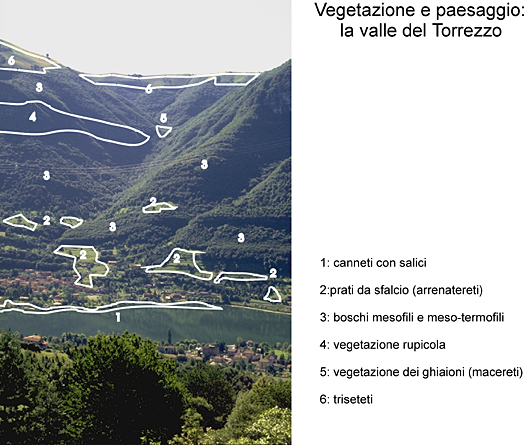
\includegraphics[width=6cm]{image5}}
\end{figure}

\begin{figure}[H]
	\centering
	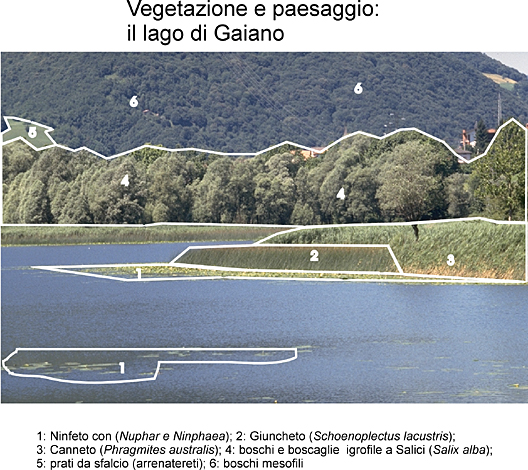
\includegraphics[width=0.4\textwidth]{image2}
	\caption{Lago di Gaiano}
	\label{fig:fotolago}
\end{figure}




Nella \cref{fig:fotolago} possiamo vedere delle fotografie raffiguranti il lago. Notiamo nel dettaglio 3 viste in cui possiamo notare la collazione dei vari tipi di vegetazione.

\begin{wrapfigure}[9]{r}{0.5\textwidth}
	\centering
	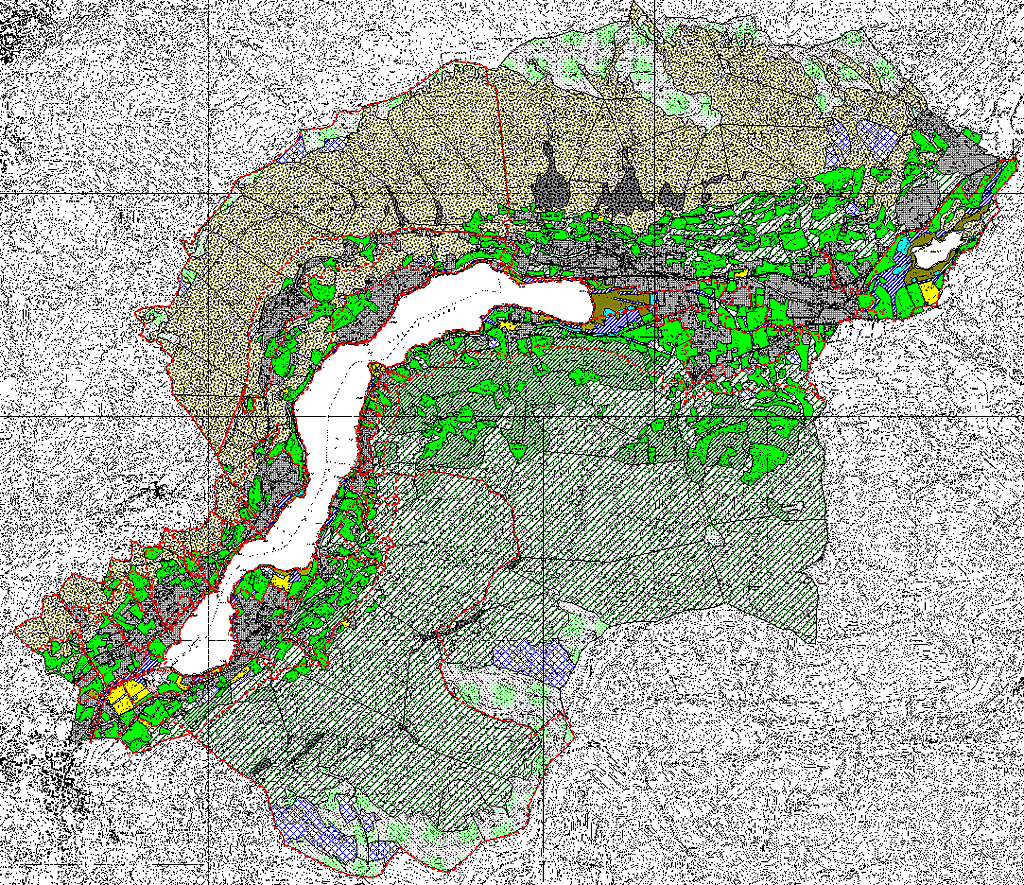
\includegraphics[width=0.4\textwidth]{image44}
	\caption{Carta della vegetazione del PLIS}
\end{wrapfigure}

Le acque, sufficientemente limpide, tendono ad un caratteristico colore verde scuro. Il perimetro del lago è totalmente percorribile.

\subsection{Vegetazione autoctona}




L'area dei laghi di Endine si contraddistingue per la presenza di formazioni igrofile e palustri. Verso le rive sono presenti fasce di ninfeti costituiti da Ninfa e Ninfa gialla, cui sono associate altre specie tra cui il Ranuncolo d’acqua.



Il lago è circondato da una fascia quasi continua di canneto, in cui abbondano sequenze costituite da Cannuccia di palude seguita da Scirpo, in posizione più esterne, e da Tifae, localizzata sulle rive. 

\begin{wrapfigure}[20]{r}{0.5\textwidth}
	\centering
	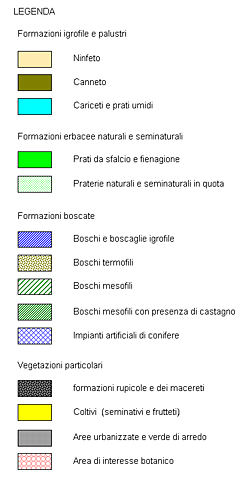
\includegraphics[width=0.4\textwidth]{image18}
	\caption{Legenda}
\end{wrapfigure}

Ai margini delle aree lacustri, o lungo alcuni piccoli immissari, sono presenti formazioni boscate igrofile nelle quali si possono osservare Ontani neri, Frassini maggiori, Pioppi neri, Salici bianchi e raramente Platani. Nello strato arbustivo si segnala la presenza di Sanguinella, Sambuco, Aglio orsino, Rovi, Oppio, Ortica mora e Canapa acquatica.  Nei siti più vicini all'acqua sono osservabili anche Noccioli, Biancospini , Salici, Ontani neri, Frangola e Dulcamara. Sui versanti meno soleggiati sono presenti formazioni boscate mesofile, costituite da specie quali aceri di monte, Frassini maggiori, Carpini bianchi , Ciliegi selvatici, Conifere, Castagneti e Faggi ad alte quote.  Sui fianchi ben assolati e meglio esposti attorno al lago sono insediate formazioni boscate termofile dove si osservano Carpini neri, Roverelle e Ornielli.

\pagebreak
	\newpage
	\section{Struttura precedente}

La struttura sulla quale mi sono basato per il mio progetto si trova sul lago di Endine  precisamente nel comune di Spinone in via Nazionale 56. 

\begin{figure}[H]
	\centering
	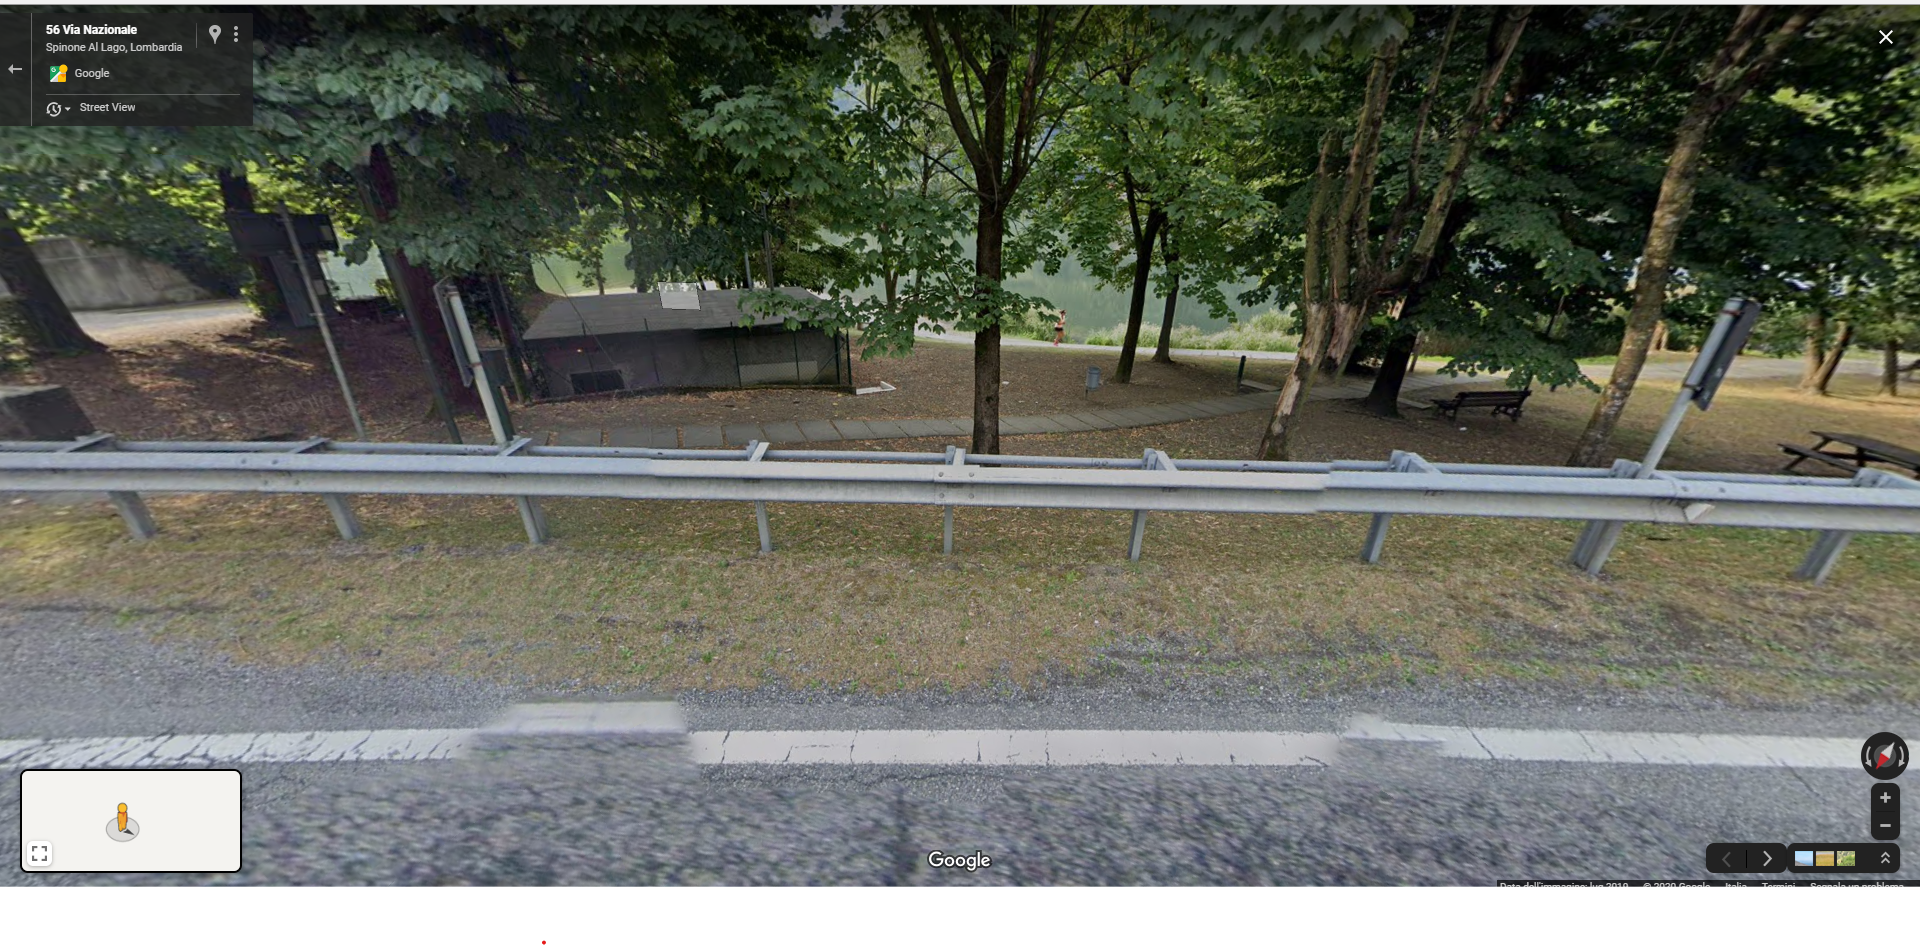
\includegraphics[width=0.8\textwidth]{image11}
	\caption{aaa}
	\label{fig:mesh1}
\end{figure}



Si tratta di  un edificio privato,dalle dimensioni di 4,30 x 5,40 metri, che in precedenza era adibito a rimessaggio per le barche.
Mi ha interessato la sua posizione perché dista pochi metri dal lago, è immersa in un ampio spazio verde, alberato  e situata di fronte alla pista pedonale.
Si tratta di un passaggio molto frequentato  che permette di percorrere tutto il lago. 
Nei periodi estivi e di bella stagione diventa un luogo di svago e relax per famiglie e gruppi di compagnie.
La zona circostante è pubblica ed è già allestita con tavoli e panchine.
Alle spalle passa un vialetto  che si congiunge alla strada principale, permettendo di raggiungere facilmente la struttura e offrendo dei parcheggi.

\subsection{Collocazione}

L’edificio per il rimessaggio si trova sul versante ovest del lago. Gode di un'ottima posizione ed esposizione alla luce solare.

\begin{figure}[H]
	\captionsetup[subfloat]{farskip=2pt,captionskip=8pt}
	\centering
	\subfloat[Mappa]{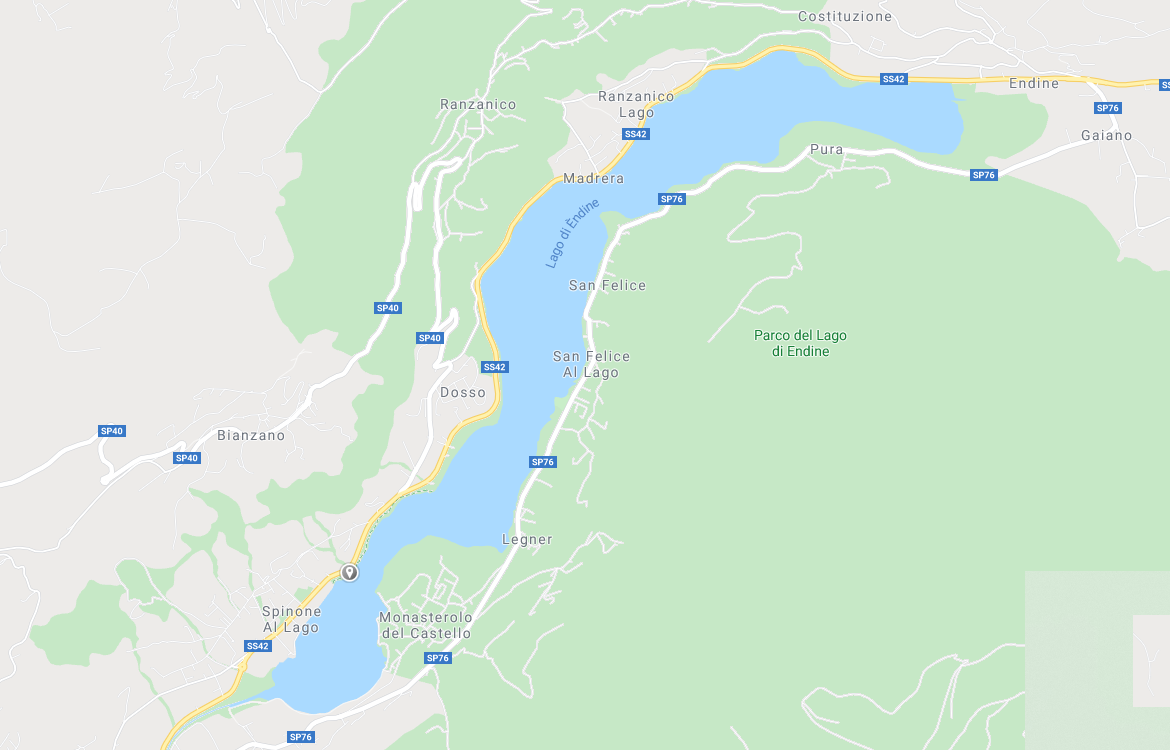
\includegraphics[width=6cm]{image12}}
	\hspace{1cm}
	\subfloat[Mappa aerea]{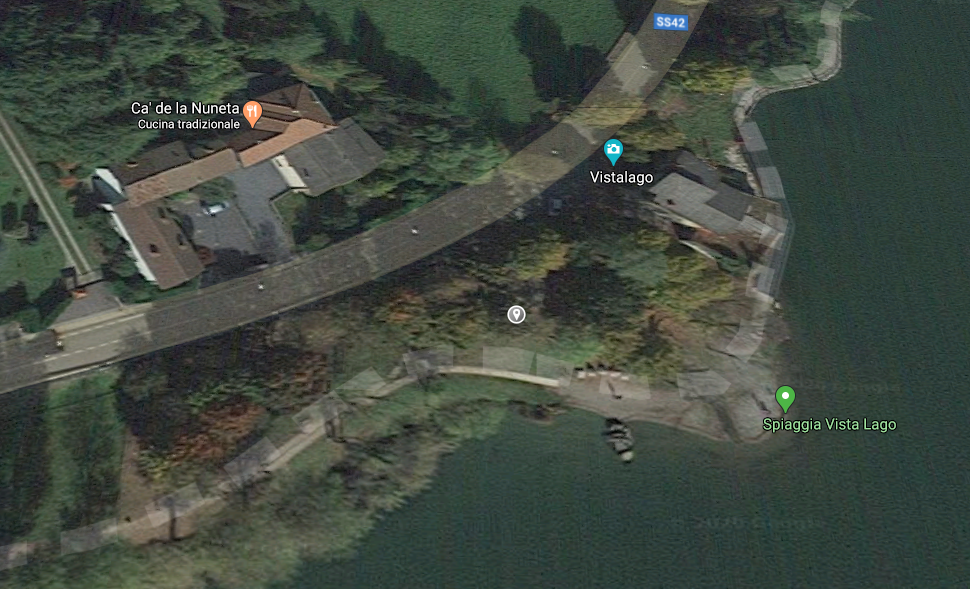
\includegraphics[width=6cm]{image24}}
	
	\caption{Mappe}
	\label{fig:imagesizes}
\end{figure}


\begin{figure}[H]
	\centering
	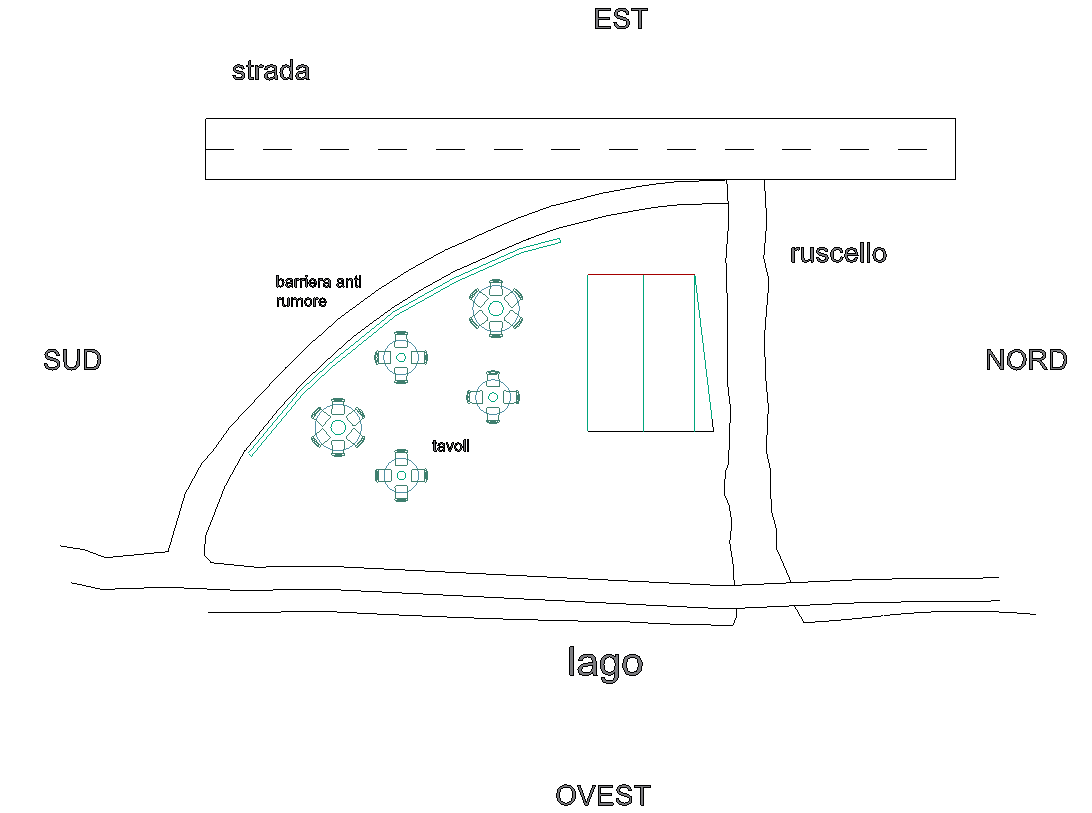
\includegraphics[width=0.8\textwidth]{image45}
	\caption{aaa}
	\label{fig:mesh1}
\end{figure}
	\newpage
	\section{Regolamento Comune}

L’installazione su area pubblica di un chiosco per la vendita di giornali o per la somministrazione al pubblico di alimenti e bevande richiede, oltre all’autorizzazione per l’occupazione di suolo pubblico e a quella per l’attività commerciale anche il permesso di costruire di cui al DPR 380/01.


\paragraph{Art. 3 (L) - Definizioni degli interventi edilizi} ~\\
\noindent
Ai fini del presente testo unico si intendono per: \textit{"interventi di ristrutturazione edilizia"}, 

\begin{enumerate}[a)]
	\item gli interventi di nuova costruzione;gli interventi rivolti a trasformare gli organismi edilizi mediante un insieme sistematico di opere che possono portare ad un organismo edilizio in tutto o in parte diverso dal precedente. Tali interventi comprendono il ripristino o la sostituzione di alcuni elementi costitutivi dell'edificio, l’eliminazione, la modifica e l'inserimento di nuovi elementi ed impianti. Nell'ambito degli interventi di ristrutturazione edilizia sono ricompresi anche quelli consistenti nella demolizione e ricostruzione con la stessa volumetria di quello preesistente, fatte salve le sole innovazioni necessarie per l'adeguamento alla normativa antisismica nonché quelli volti al ripristino di edifici, o parti di essi, eventualmente crollati o demoliti, attraverso la loro ricostruzione, purché sia possibile accertarne la preesistente consistenza. 
\end{enumerate}
\paragraph{Art. 10 (L) - Interventi subordinati a permesso di costruire} ~ \\
\noindent
Costituiscono interventi di trasformazione urbanistica ed edilizia del territorio e sono subordinati a permesso di costruire:
\begin{enumerate}[a)]
	\item gli interventi di nuova costruzione;
	\item gli interventi di ristrutturazione urbanistica
	\item gli interventi di ristrutturazione edilizia che portino ad un organismo edilizio in tutto o in parte diverso dal precedente e che comportino modifiche della volumetria complessiva degli edifici o dei prospetti, ovvero che, limitatamente agli immobili compresi nelle zone omogenee A, comportino mutamenti della destinazione d’uso, nonché gli interventi che comportino modificazioni della sagoma di immobili sottoposti a vincoli ai sensi del decreto legislativo 22 Gennaio 2004, n. 42 e successive modificazioni.
\end{enumerate}
	\newpage
	\section{Idea Progettuale}

\subsection{Ispirazione}

Visitando frequentemente questo luogo, che affascina per la presenza del lago. È stato pensato quindi di poter riconvertire il rimessaggio barche in un bar/chiosco (\cref{fig:stuttura}). Vista la sua collocazione é stato immaginato che il bar potesse offrire anche un servizio \textit{take-away} e cestini merenda da consumare in riva al lago. In questo modo si può compensare la quantità di tavoli disponibili, soprattutto nei periodi più ad alta affluenza. 

\begin{wrapfigure}[18]{r}{0.5\textwidth}
	\centering
	
\includegraphics[width=0.4\textwidth]{image14}
	\caption{Struttura}
	\label{fig:stuttura}
\end{wrapfigure}

Trattandosi di una struttura semi aperta la quantità di tavoli disponibili è limitata; allo stesso tempo alcuni clienti potrebbero non essere propensi a dover consumare il pasto direttamente in loco in quanto sarebbero inclini ad utilizzare gli spazi verdi circostanti. Dare la possibilità del \textit{food-to-go} ci viene a vantaggio per 2 motivi, in primo luogo andiamo ad ampliare il bacino di utenti ed al contempo si possono servire più pasti non dovendosi preoccupare della quantità di tavoli disponibili; in secondo luogo il servizio \textit{take-away} porterebbe ad una riduzione totale del prezzo del servizio se questa modalità è scelta. In questo modo il cliente, che in caso di servizio al tavolo non avrebbe consumato, è invogliato sia dal prezzo minore che dal \say{vantaggio} di poter consumare in libertà. Lato commerciante questo servizio permette una riduzione dei costi di pulizia e, seppur in modo minore, del trattamento dei rifiuti.  Per questi motivi il servizio di \textit{take-away} potrebbe essere molto vantaggioso a livello commerciale.

L'obbiettivo è stato quello di realizzare una struttura  originale, che non fosse troppo statica e che non  stridesse con l’ambiente circostante . Non volevo un posto totalmente chiuso . Ho quindi individuato un progetto (\cref{fig:stuttura}) che,  con  le sue due  pareti libere,  permettesse di avere sempre la visione del lago e desse la sensazione di essere in uno spazio aperto. 

\clearpage
\subsection{Struttura}


La struttura, larga $4.30$ metri e lunga $5.40$ metri, è costruita con legno di larice come rivestimento(\cref{fig:listelli}), travi  d'acciaio \textit{IPE}  e chiusure trasparenti.

\begin{wrapfigure}[11]{r}{0.5\textwidth}
	\centering
	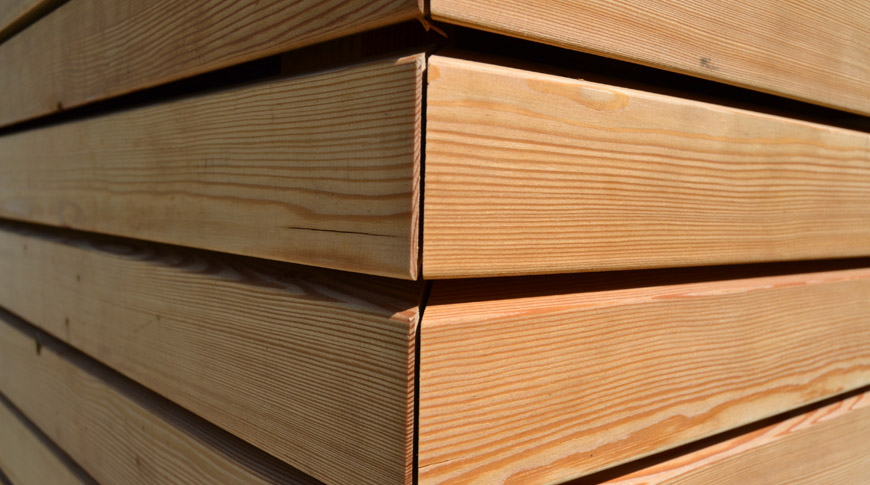
\includegraphics[width=0.4\textwidth]{image21}
	\caption{Listelli in legno}
	\label{fig:listelli}
\end{wrapfigure}

l legno di larice è un ottimo legno per rivestimenti per esterni, grazie alle sue notevoli proprietà isolanti. Il legno di larice tende ad assumere una tonalità grigiastra con il passare del tempo e tale escursione cromatica che lo rende particolarmente apprezzato . Inoltre ha una notevole durezza, resistenza alle sollecitazioni e un buon coefficiente di impermeabilità. 

Il lato nord è costituito da una parete di legno con due diverse inclinazioni; anche il lato ovest ,che si rivolge alla strada, è costituito da una parete di legno, mentre i lati est e sud sono aperti. Tutta la struttura poggia su una pedana di legno. I due lati aperti permettono il diretto accesso al bancone del bar e rendono la struttura integrata con l’ambiente che la circonda. 

La struttura è pensata per un uso estivo, visto che non offre tavoli al coperto. 
Ho previsto una chiusura dei lati aperti tramite una serranda orizzontale, 
in modo da chiudere il chiosco durante la notte o durante il periodo di non utilizzo. 

\begin{figure}[H]
	\centering
	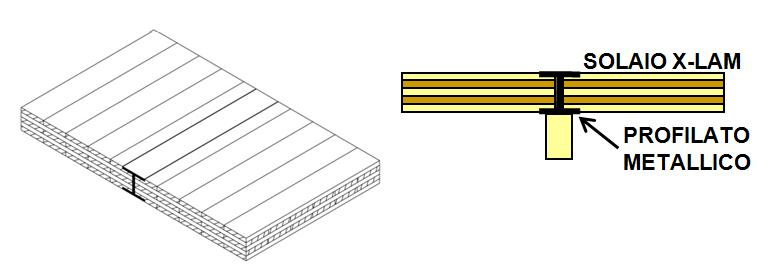
\includegraphics[width=0.8\textwidth]{image35}
	\caption{Interna struttura}
	\label{fig:pedana}
\end{figure}

\clearpage
La parte frontale della struttura si sviluppa a partire dalla forma di un pentagono, mentre la parte posteriore relativa ad un guscio di protezione. La scelta di di utilizzare un pentagono (\cref{fig:pentagono}) é stata pensata in modo da suddividere la struttura in due zone. Essa consente di avere una parte protettiva esterna; allo stesso tempo il lato opposto presenta un apertura verso l'ambiente lacustre.

\begin{figure}[H]
	\captionsetup[subfloat]{farskip=2pt,captionskip=8pt}
	\centering
	\subfloat[Vista laterale]{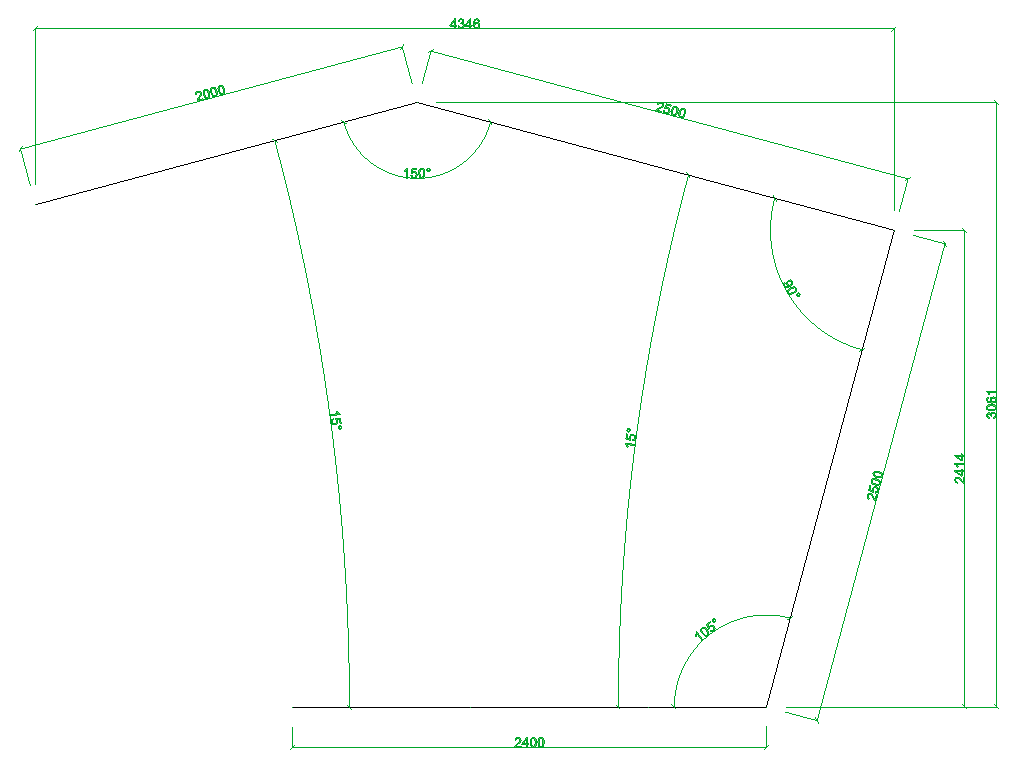
\includegraphics[width=6cm]{image43}}
	\hspace{1cm}
	\subfloat[Vista posteriore]{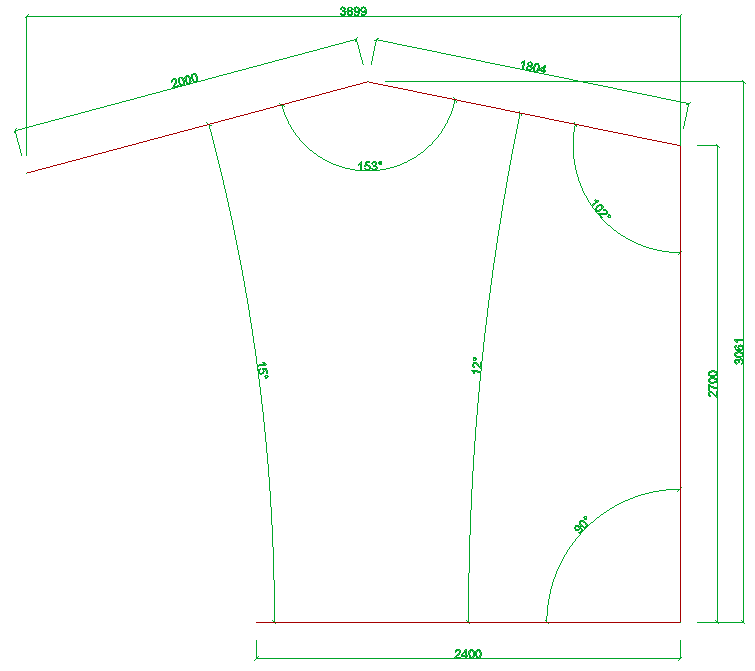
\includegraphics[width=6cm]{image1}}
\end{figure}

\begin{figure}[H]
	\captionsetup[subfloat]{farskip=2pt,captionskip=8pt}
	\centering
	\subfloat[Vista laterale: Guscio di protezione]{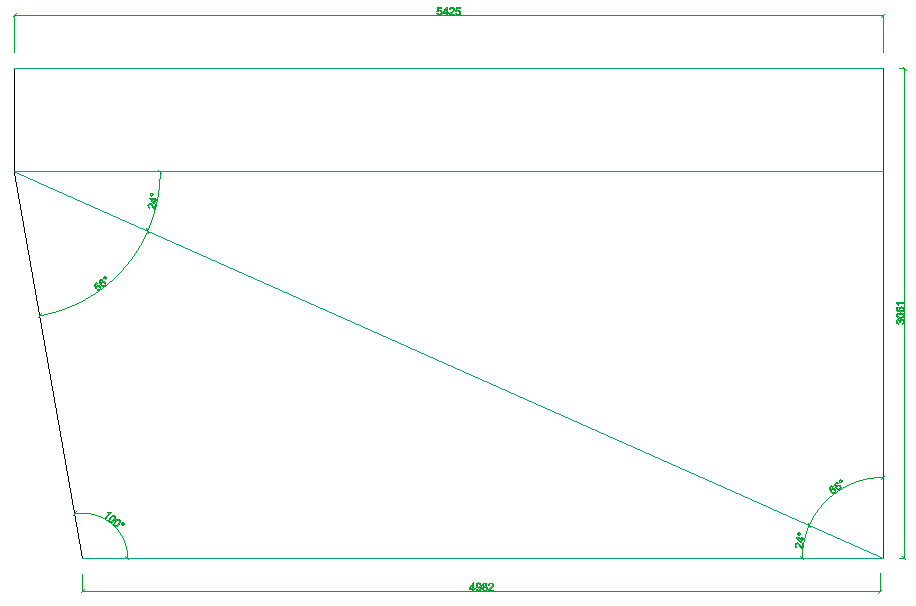
\includegraphics[width=6cm]{image34}}
	\hspace{1cm}
	\subfloat[Prospetto posteriore]{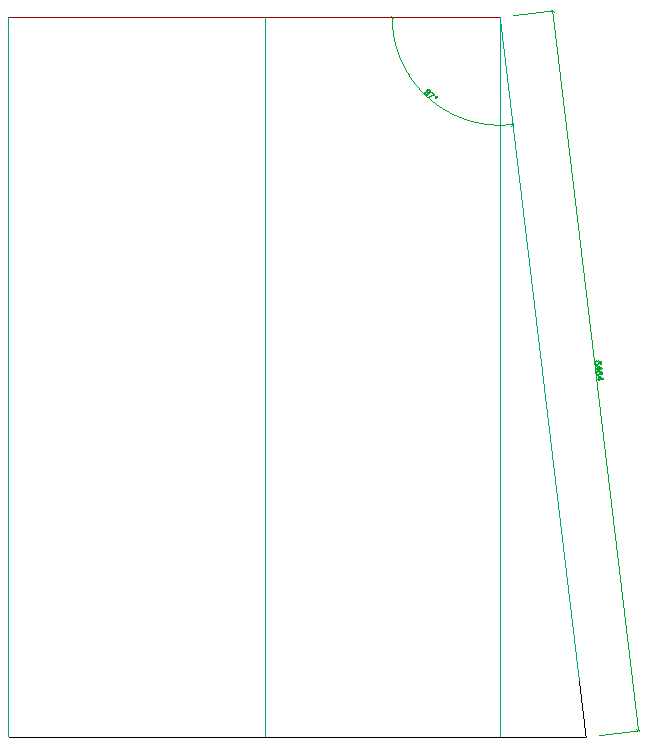
\includegraphics[width=6cm]{image32}}
	
	\caption{Viste}
	\label{fig:pentagono}
\end{figure}




\subsection{Analisi delle indicazione ergonomiche relative ai moduli costituenti il bancone da lavoro }

Il bar può essere suddiviso in quattro sotto-aree funzionali: piano di servizio, piano di lavoro, sotto banco  e retrobanco.

Il piano di servizio è posizionato poco più in alto rispetto a quello di lavoro. Può essere rivestito nel materiale che si preferisce, in linea con lo stile del locale. 
È l’elemento di comunicazione tra cliente e barista ed è l’area dove vengono servite le preparazioni e disposti gli snack per gli aperitivi. L'altezza totale del banco equivale all'altezza della bancalina, generalmente realizzata in marmo/pietra/corian o acciaio  ($\sim  1150mm$ da terra). In \cref{fig:persone} possiamo vedere una sezione del bancone in rapporto a due figure in modo da contestualizzare le misure.

\begin{figure}[H]
	\centering
	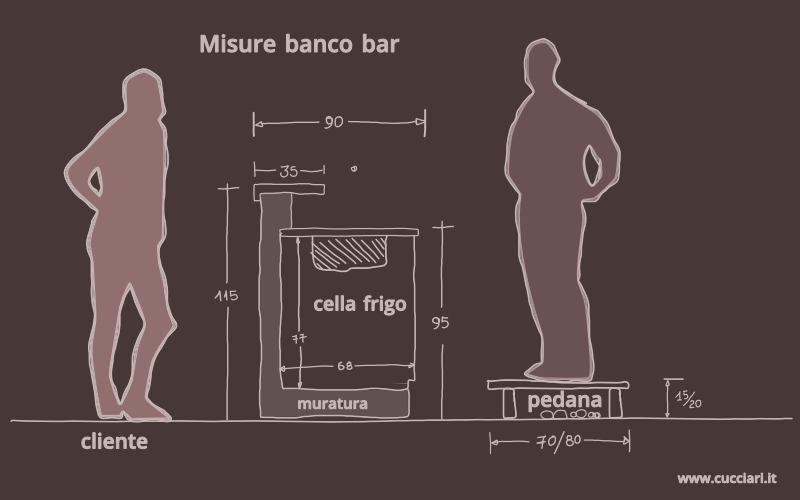
\includegraphics[width=0.6\textwidth]{image39}
	\caption{Banco bar con figure}
	\label{fig:persone}
\end{figure}

\noindent
Il piano di lavoro è la parte in cui vengono posizionate le attrezzature del bar utilizzate più spesso e meno ingombranti ed è appunto la zona in cui il barista prepara bevande e snack. L’altezza del piano di lavoro è di  $950mm$ da terra, in genere realizzato in acciaio inox. È qui che generalmente trova posto anche il lavello con acqua corrente e uno spazio per bottiglie di uso frequente.


Nel sottobanco trovano posto tutte quelle attrezzature più ingombranti, utilizzate quotidianamente e adibite soprattutto alla conservazione delle bevande e al lavaggio: tra questi il frigorifero, la macchina per il ghiaccio, la lavabicchieri o la lavastoviglie professionale. L'apertura dei vani refrigerati avviene attraverso sportelli o cassetti, interamente  in acciaio inox. Nel retrobanco del bar viene allestito il reparto caffetteria e espositore. Il retrobanco può essere neutro o refrigerato e composto da un numero variabile di armadietti con sportelli o cassetti, si possono dividere più o meno in due parti. Generalmente si distingue in due sezioni principali:


\begin{figure}[H]
	\captionsetup[subfloat]{farskip=2pt,captionskip=8pt}
	\centering
	\subfloat[Retro espositivo]{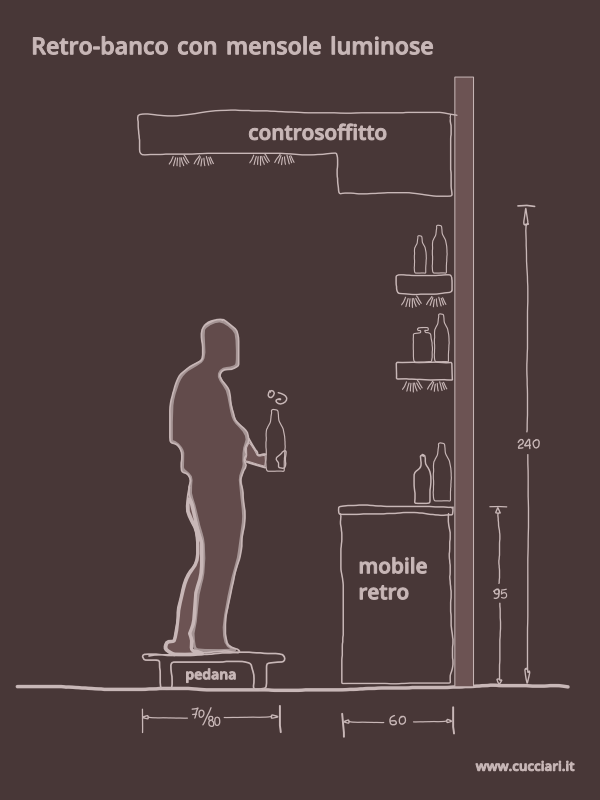
\includegraphics[width=6cm]{image46}}
	\hspace{1cm}
	\subfloat[Retro macchina caffè]{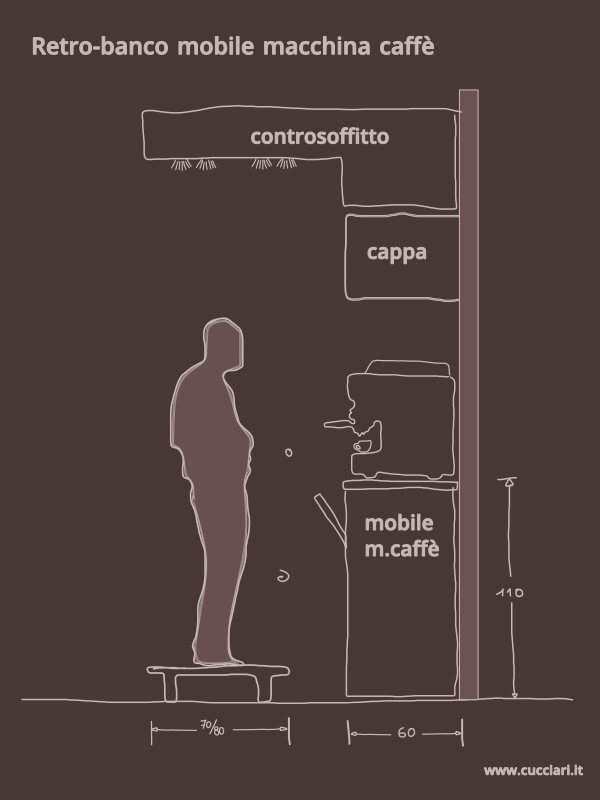
\includegraphics[width=6cm]{image8}}
	
	\caption{Retrobancone}
	\label{fig:imagesizes}
\end{figure}

\noindent
Retro multiuso e bottiglie.  Composto da una base e da un'alzata su cui si applicano le mensole portabottiglie o i fondali attrezzati per vari servizi. Qui troviamo: cassetti, macina-caffè,  tramoggia per i fondi del caffè, spazzatura, uno spazio per la lavastoviglie oppure il produttore di ghiaccio, un vano per l’addolcitore ed infine la pompa macchina caffè.


	\newpage
	\section{Utilizzo degli spazi nel chiosco interno ed esterno}

\begin{figure}[H]
	\centering
	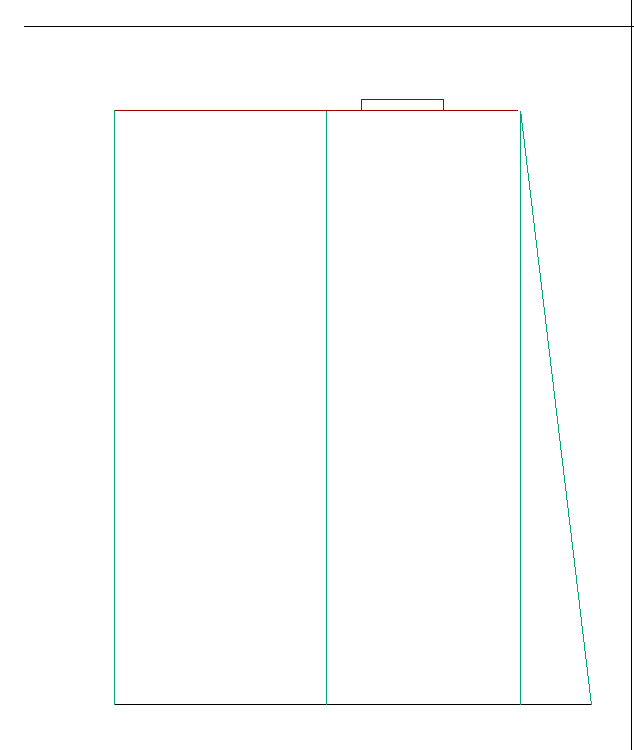
\includegraphics[width=0.5\textwidth]{image42}
	\caption{Vista struttura}
	\label{fig:mesh1}
\end{figure}


\begin{figure}[H]
	\centering
	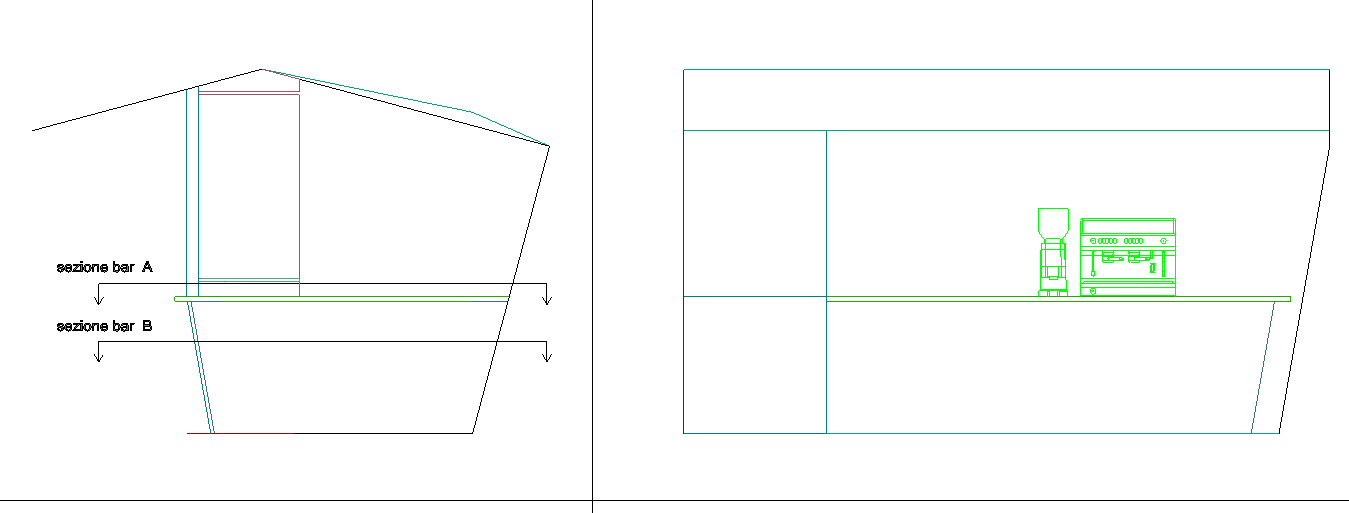
\includegraphics[width=0.8\textwidth]{image23}
	\caption{aaa}
	\label{fig:mesh1}
\end{figure}


\subsection{Progettazione bancone}


\begin{figure}[H]
	\centering
	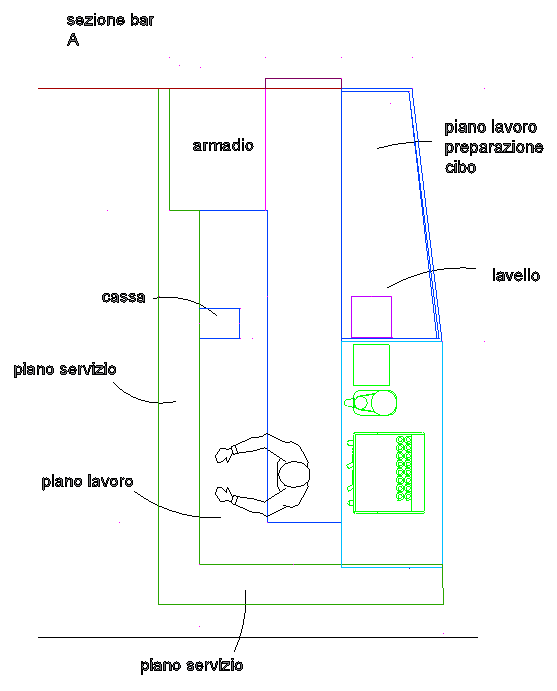
\includegraphics[width=0.5\textwidth]{image29}
	\caption{Progettazione bancone}
	\label{fig:mesh1}
\end{figure}

Nell'immagine  possiamo vedere la composizione del bar  , dove troviamo un'area di lavoro divisa in due. La parte di ordini/cassa e preparazione del cibo  e la parte caffetteria/ distribuzione bibite.

\begin{figure}[H]
	\centering
	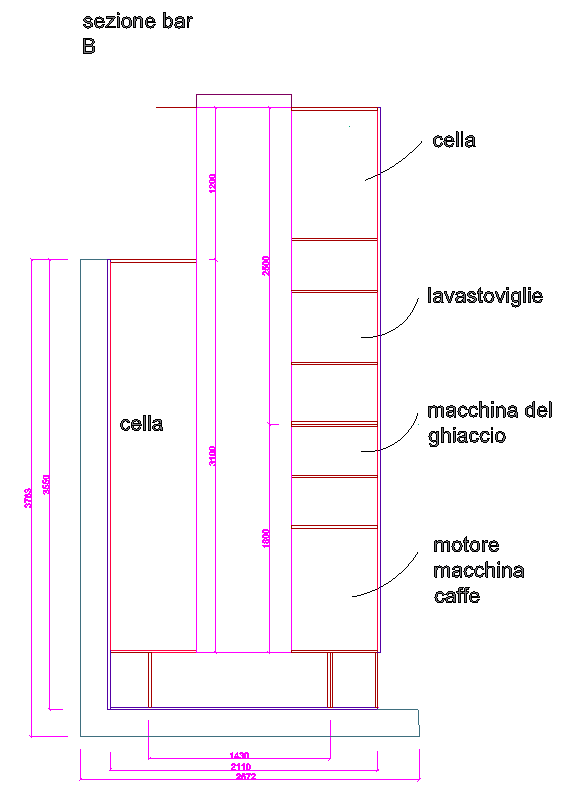
\includegraphics[width=0.5\textwidth]{image13}
	\caption{Sezione bar B}
	\label{fig:mesh1}
\end{figure}

sezione B
Qui possiamo vedere come ho gestito la divisione dei moduli.
Sul lato sinistro troviamo un armadio da 1200 mm e uno spazio dove collocare una cella da 3000 mm .
Sul lato opposto troviamo un modulo dalla lunghezza totale di 4300 mm 
Uan  altro piccolo modulo di 1430mm disposto perpendicolare a questi due chiude la zona lavoro. 

\begin{figure}[H]
	\centering
	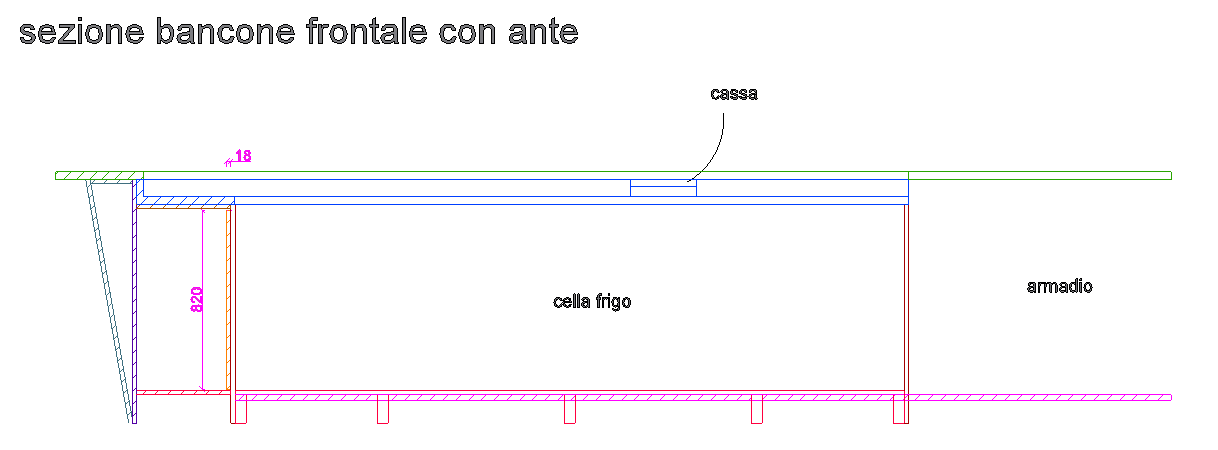
\includegraphics[width=0.8\textwidth]{image4}
	\caption{Sezione bancone frontale con ante}
	\label{fig:mesh1}
\end{figure}


Possiamo vedere in verde le misure del bancone di servizio ed in blu il piano di lavoro dove è anche collocata la  cassa  ed in fine il vano per la cella dalla lunghezza di 3000 mm . 
Il vano a destra è riservato alla collocazione di un armadio su misura. 

\begin{figure}[H]
	\centering
	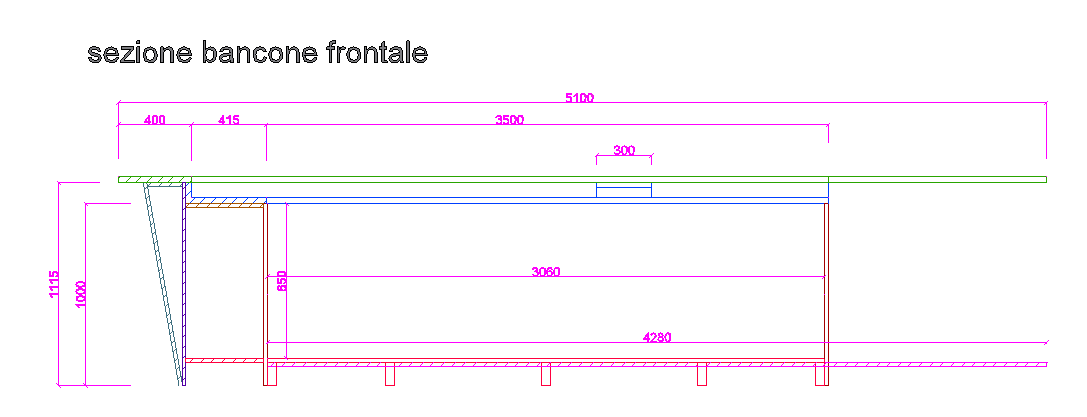
\includegraphics[width=0.8\textwidth]{image20}
	\caption{Sezione bancone frontale}
	\label{fig:mesh1}
\end{figure}

\begin{figure}[H]
	\centering
	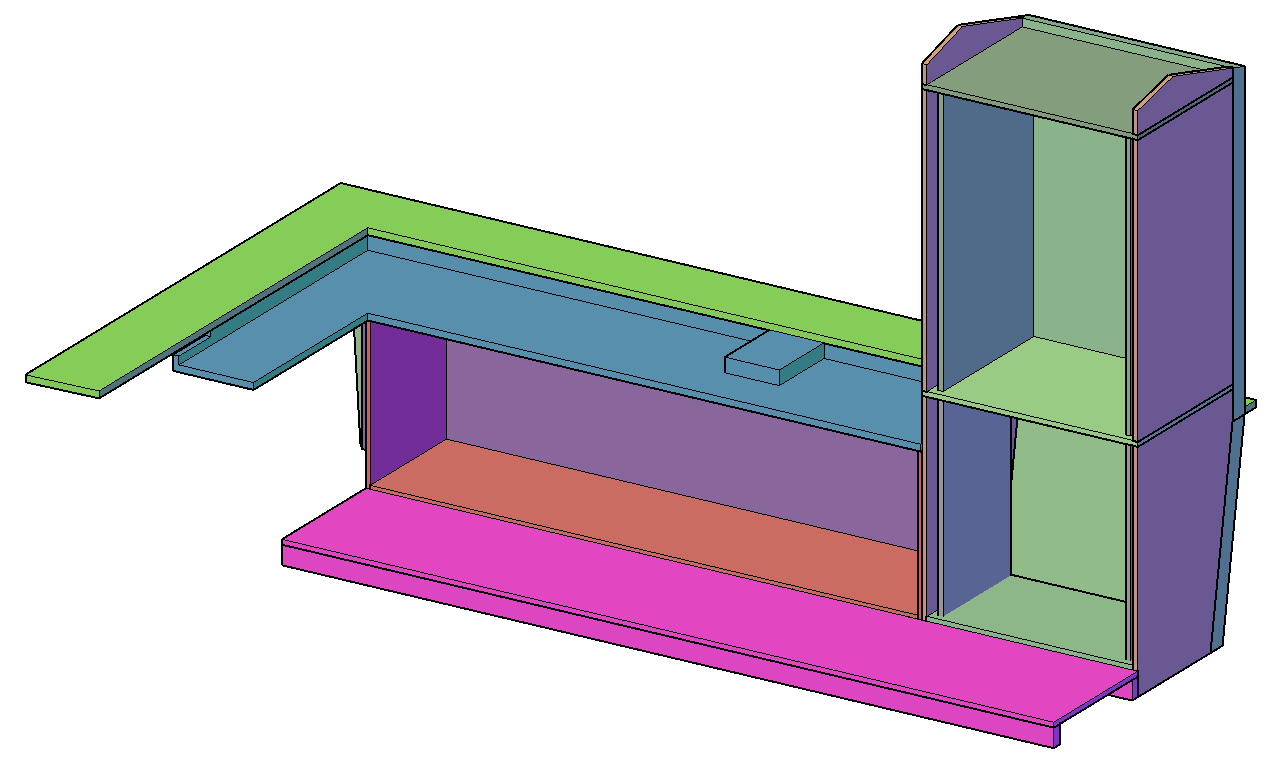
\includegraphics[width=0.8\textwidth]{image26}
	\caption{Sezione bar A}
	\label{fig:mesh1}
\end{figure}

Il primo modulo da $2500mm$ contiene una cella da $1000 mm$, un piccolo armadietto, un vano riservato alla lavastoviglie, un altro piccolo armadietto e il vano dove sarà inserito il lavello.

\begin{figure}[H]
	\centering
	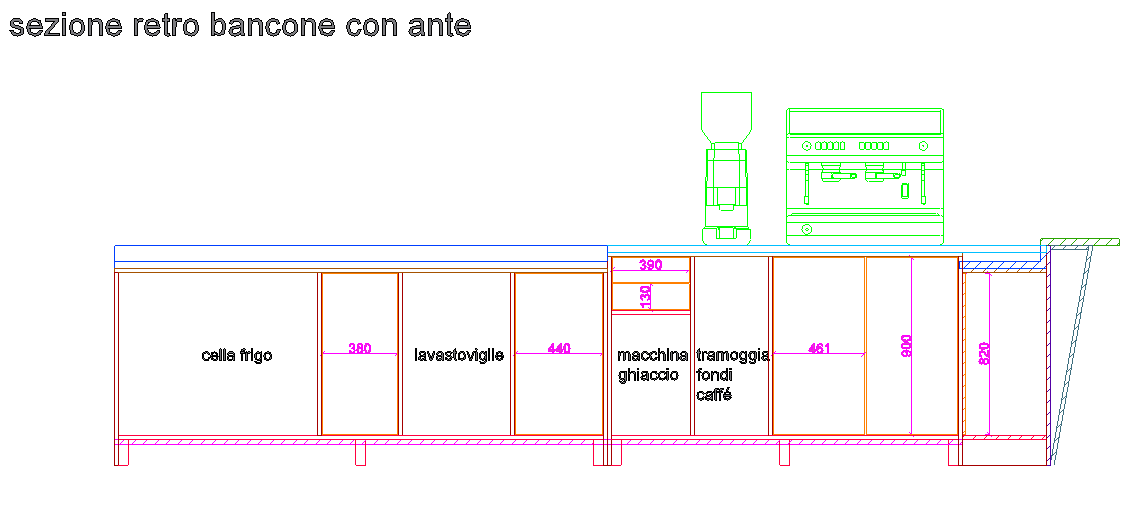
\includegraphics[width=0.8\textwidth]{image41}
	\caption{???}
	\label{fig:mesh1}
\end{figure}

Il secondo modulo da $1800 mm$ contiene un vano con cassetti e la macchina per il ghiaccio ,un vano tramoggia fondi caffè e spazzatura ed un armadietto a due ante dove è collocata la pompa per la macchina del caffè.

\begin{figure}[H]
	\centering
	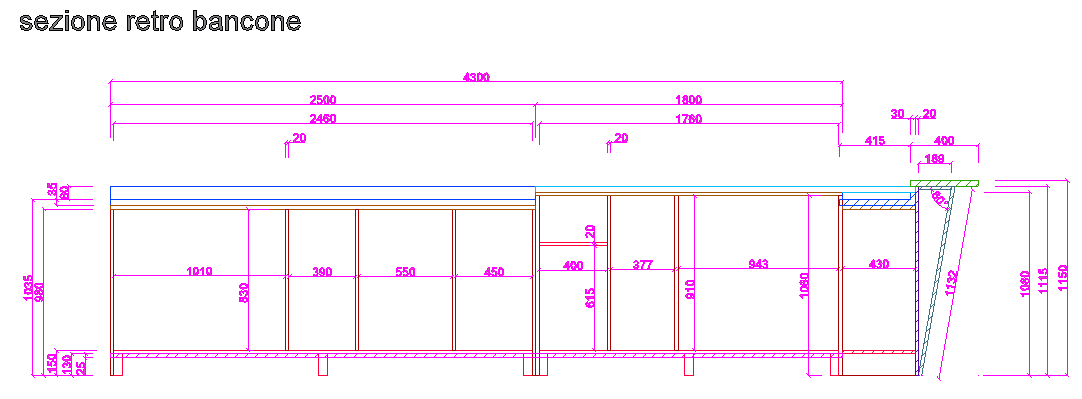
\includegraphics[width=0.8\textwidth]{image10}
	\caption{Sezione retro bancone}
	\label{fig:mesh1}
\end{figure}
\begin{figure}[H]
	\centering
	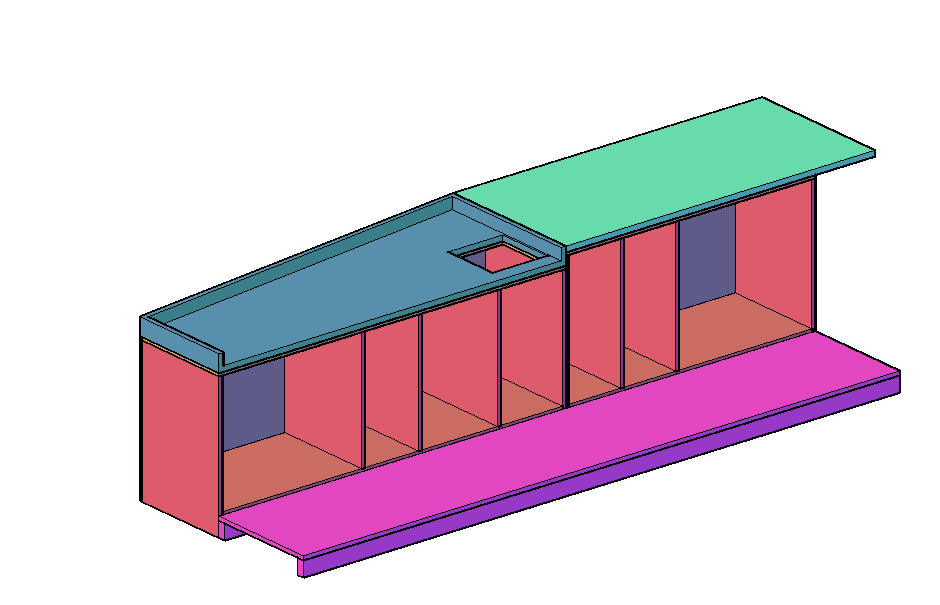
\includegraphics[width=0.8\textwidth]{image7}
	\caption{aaaa}
	\label{fig:mesh1}
\end{figure}
\begin{figure}[H]
	\centering
	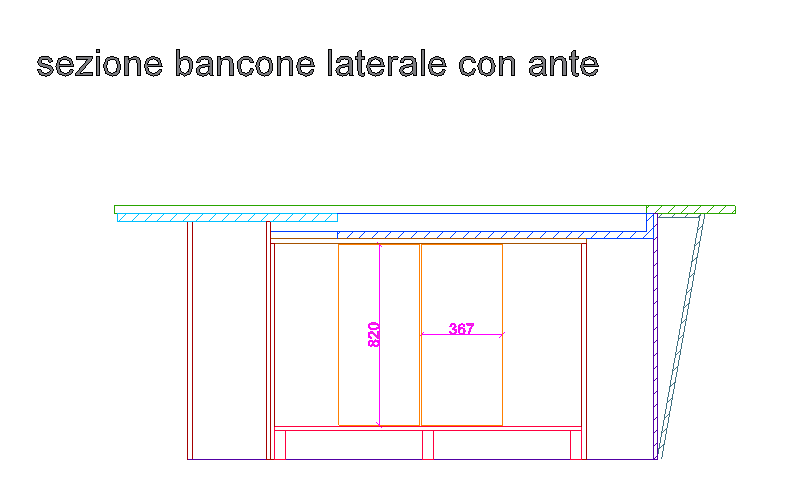
\includegraphics[width=0.8\textwidth]{image37}
	\caption{Sezione bancone laterale con ante}
	\label{fig:mesh1}
\end{figure}
\begin{figure}[H]
	\centering
	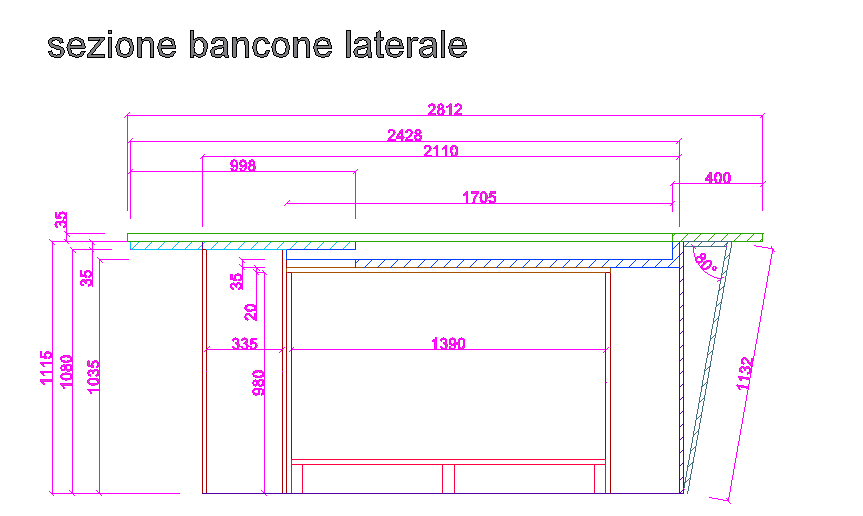
\includegraphics[width=0.8\textwidth]{image15}
	\caption{Sezione bancone laterale}
	\label{fig:mesh1}
\end{figure}
\begin{figure}[H]
	\centering
	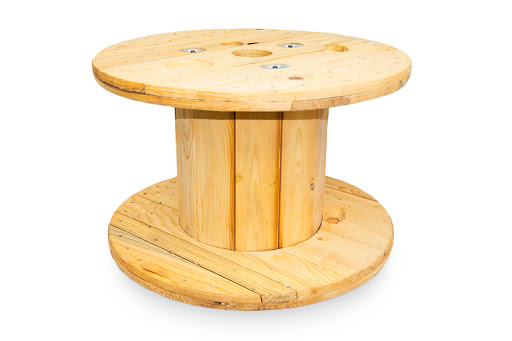
\includegraphics[width=0.8\textwidth]{image3}
	\caption{???}
	\label{fig:mesh1}
\end{figure}

\begin{figure}[H]
	\centering
	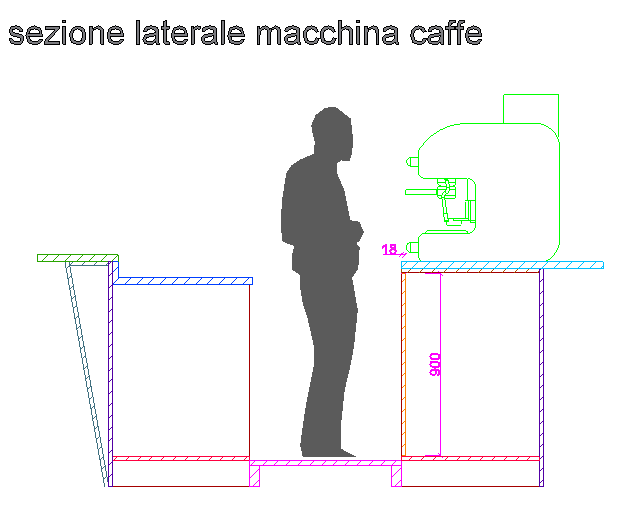
\includegraphics[width=0.8\textwidth]{image16}
	\caption{Sezione laterale macchina caffè}
	\label{fig:mesh1}
\end{figure}
\begin{figure}[H]
	\centering
	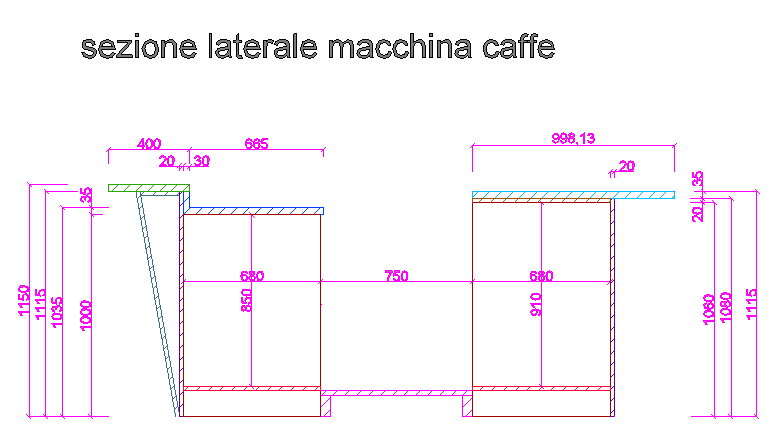
\includegraphics[width=0.8\textwidth]{image22}
	\caption{Sezione laterale macchina caffè}
	\label{fig:mesh1}
\end{figure}

\begin{figure}[H]
	\centering
	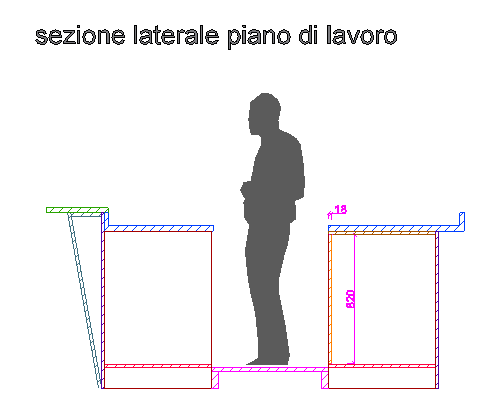
\includegraphics[width=0.8\textwidth]{image25}
	\caption{Sezione laterale piano di lavoro}
	\label{fig:mesh1}
\end{figure}

L’armadio ha una larghezza totale di 1200 mm, altezza di 3061 mm ed ha  una luce interna di 1020 mm. E’ composto da  due pezzi, una parte bassa dove troviamo il fondo in luce e il cappello che fa da fondo per la parte in alto. 
Le spalle sono composte da un fianco interno ed uno esterno. 
Come sistema di chiusura ho pensato ad un sistema a serranda orizzontale. 
Il materiale usato è multistrato  $25mm$.

\begin{figure}[H]
	\captionsetup[subfloat]{farskip=2pt,captionskip=8pt}
	\centering
	\subfloat[Vista armadio 3D]{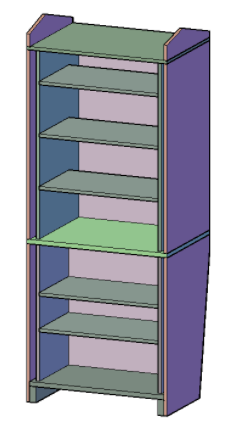
\includegraphics[width=4cm]{image57}}
	\hspace{1cm}
	\subfloat[Vista armadio]{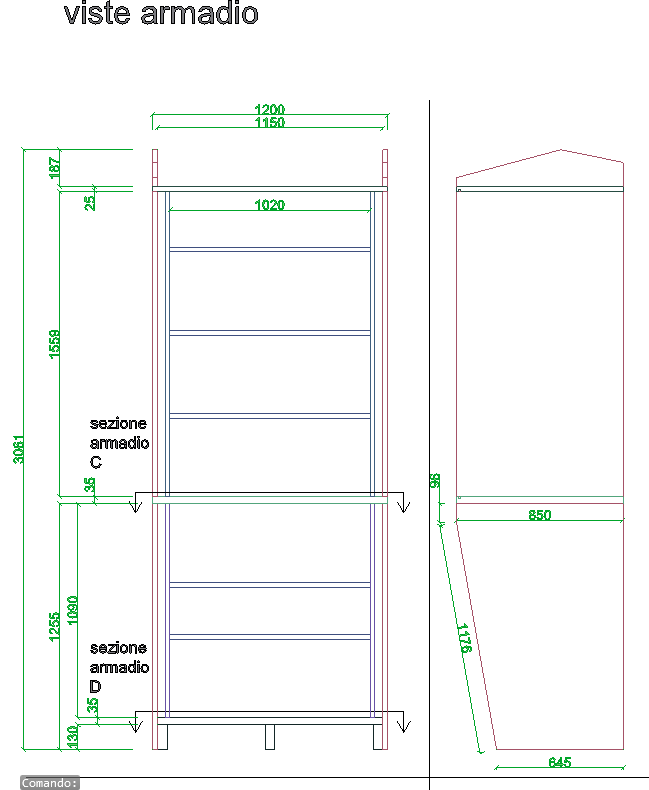
\includegraphics[width=6cm]{image19}}
	
	\caption{Armadio (sezione e vista 3D)}
	\label{fig:imagesizes}
\end{figure}

\begin{figure}[H]
	\captionsetup[subfloat]{farskip=2pt,captionskip=8pt}
	\centering
	\subfloat[Sezione laterale armadio]{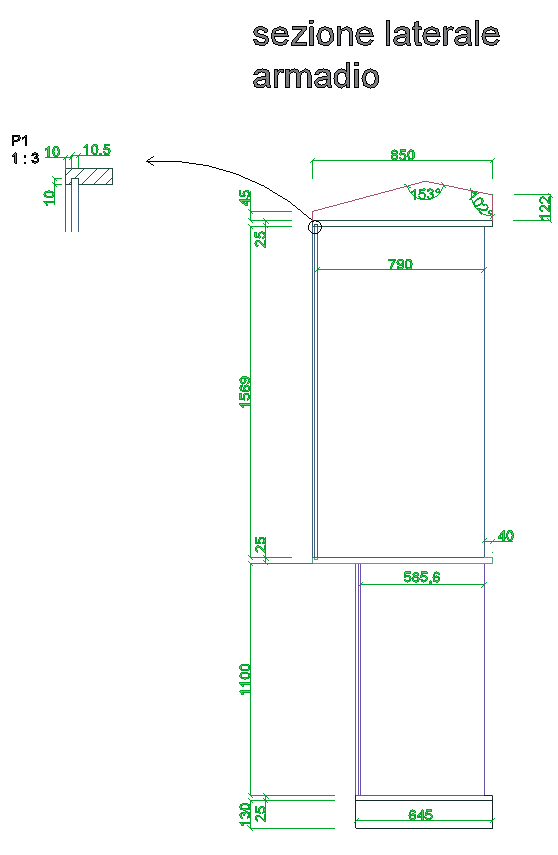
\includegraphics[width=4cm]{image6}}
	\hspace{1cm}
	\subfloat[Sezione armadio]{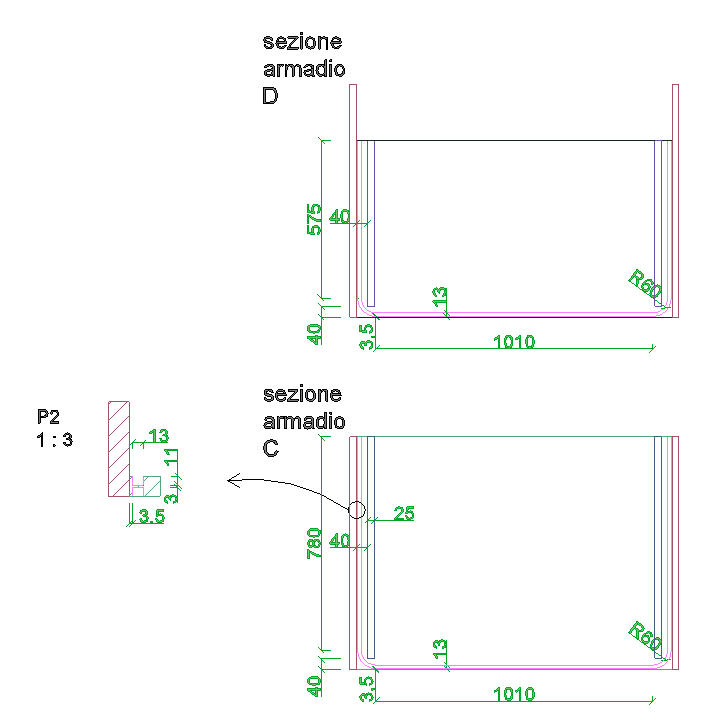
\includegraphics[width=6cm]{image30}}
	
	\caption{Sezione armadio}
	\label{fig:imagesizes}
\end{figure}


\begin{figure}[H]
	\centering
	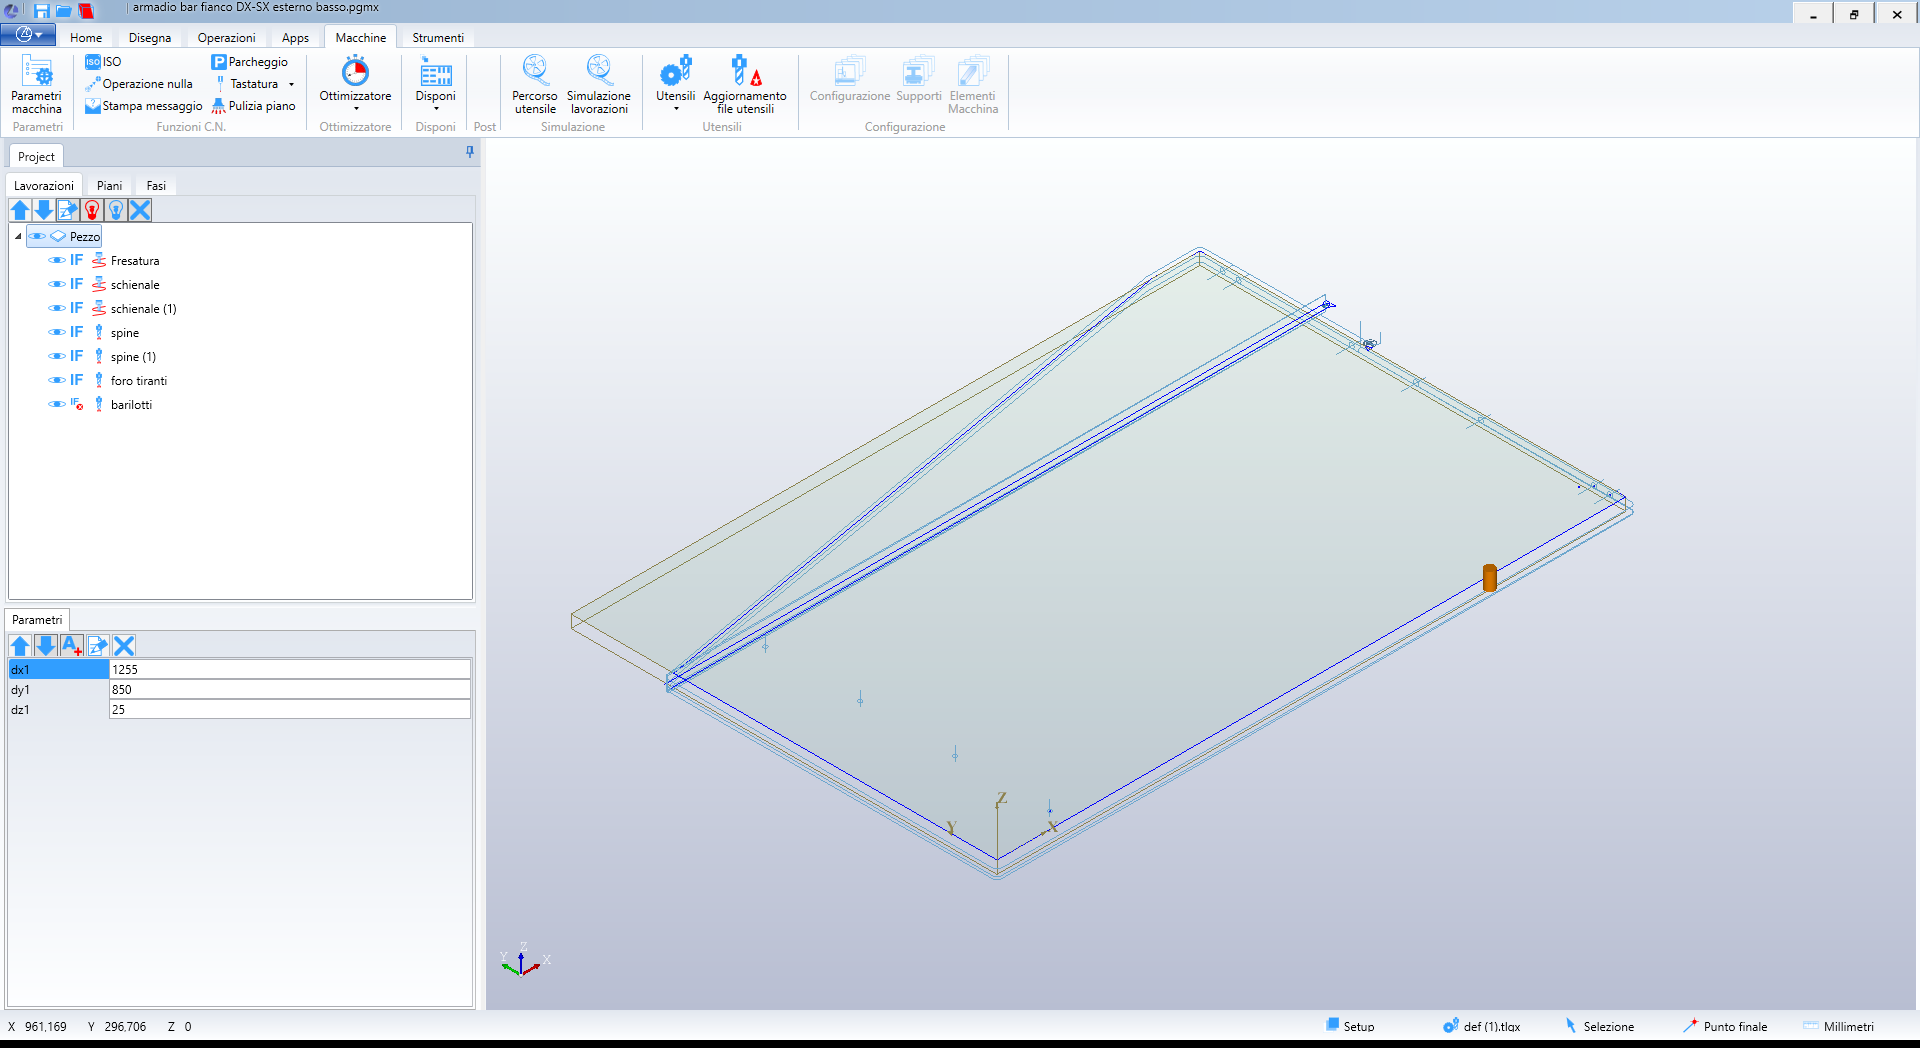
\includegraphics[width=0.8\textwidth]{image28}
	\caption{Programma PGX fianco esterno}
	\label{fig:mesh1}
\end{figure}


\section{Rafforzamento argine ruscello}

Le massicciate e le prismate sono opere di difesa spondale, realizzate con massi e/o con prismi di diverse dimensioni; gli spazi tra essi possono essere liberi o occlusi con cementi di varia natura. 
Sono preferibili le scogliere a secco, senza materiale cementante. Gli spazi permettono una migliore continuità tra fiume e falda; l’eventuale interposizione di geotessuti tra la scogliera ed il terreno retrostante consente il passaggio dell'acqua, limita il trasporto di materiali solidi, ma limita lo sviluppo delle radici delle piante colonizzatrici. 

\begin{figure}[H]
	\centering
	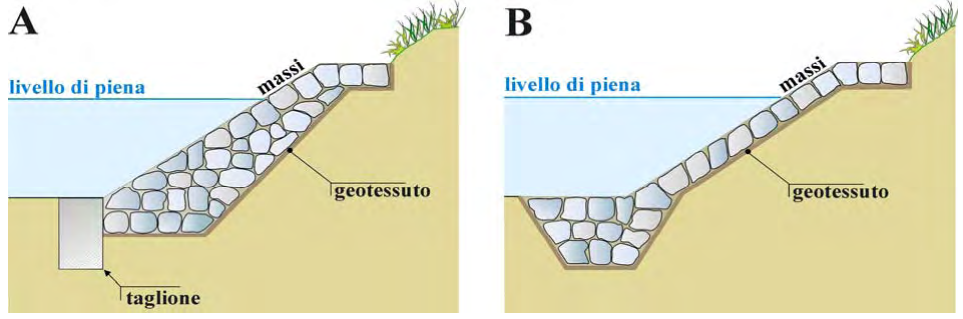
\includegraphics[width=0.8\textwidth]{image36}
	\caption{Sezione fiume}
	\label{fig:spnde}
\end{figure}

Gli spazi consentono la colonizzazione delle piante; ciò limita l’impatto sull'ecosistema e sulla qualità del paesaggio. I vegetali che crescono tra i massi ed i prismi contribuiscono, con le radici, a rendere più stabile le opere e, con le parti aeree, ad assorbire in parte l’energia delle acque di piena. Per accelerare la colonizzazione vegetale, è possibile procedere con impianti artificiali mediante talee o sistemi diversi. \\

\begin{wrapfigure}[14]{r}{0.4\textwidth}
	\centering
	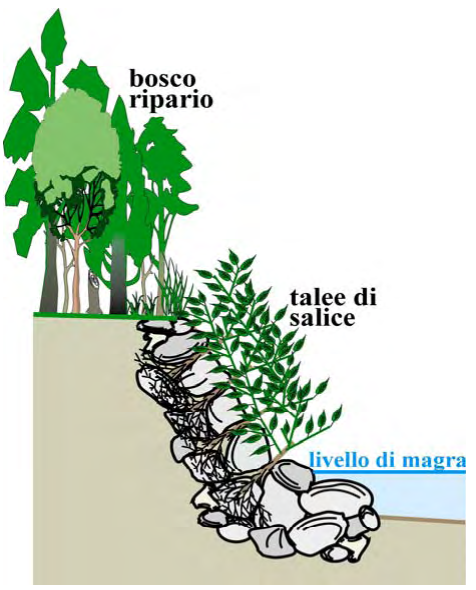
\includegraphics[width=0.3\textwidth]{image27}
	\caption{Sezione fiume}
\end{wrapfigure}

In \cref{fig:spnde} possiamo vedere le difese spondali viste in sezione: scogliera con protezione al piede (A) e mantellata con massi cementati (B).
Tali strutture sono anche denominate “massicciate” e sono caratterizzate da massi di almeno quasi una tonnellata; essi possono essere sostituiti da prismi di cemento. 


La scogliera costituisce una reale difesa puntiforme, ma che trasferisce a valle l’energia di erosione in modo tanto più efficace quanto più regolare è la geometria della scogliera stessa, soprattutto se realizzata con massi e/o prismi cementati.

\subsection{Barriera anti rumore}

Le caratteristiche acustiche di una barriera antirumore possono essere classificate in due categorie: 
\begin{itemize}
	\item estrinseche: efficienza della barriera antirumore nel ridurre i livelli di pressione sonora in una serie di punti sul territorio, chiamati recettori
	\item intrinseche: caratteristiche proprie del “prodotto” barriera antirumore, indipendentemente dall'ambiente in cui è o sarà installato e dall'effetto finale di riduzione del rumore sui ricettori (assorbimento/riflessione, trasmissione, diffrazione del suono).
\end{itemize}


Esistono numerose tipologie di barriere acustiche e di materiali componenti. La scelta di un prodotto dipende, oltre che dalle prestazioni acustiche richieste, anche da fattori, quali: statica, sicurezza, estetica, durata, manutenzione, costi. Le barriere antirumore possono essere suddivise nelle seguenti tipologie: 

\begin{enumerate}
	\item Barriere Artificiali
	\begin{itemize}
		\item Fonoisolanti (struttura alveare)
		\item Fonoassorbenti 
		\item Fonoisolanti e fonoassorbenti
	\end{itemize}
	
	\item Barriere Naturali
	\begin{itemize}
		\item Barriere vegetali (siepi, fasce boscate, alberate) 
		\item Barriere miste (terre armate, biomuri, muri verdi, barriere vegetative)
	\end{itemize}
\end{enumerate}


\subsection{Come l’ho realizzata}

ho deciso di realizzare una barriera antirumore per riparare il chiosco dalla strada molto trafficata, la barriera sarà divisa in due:
La parte esterna, rivolta verso il traffico, sarà realizzata con pannelli in lamiera di acciaio o di alluminio. L'interno dei pannelli ospita uno strato alveolare e un materiale fibroso fonoassorbente che combina attenuazione, isolamento ed assorbimento in una struttura modulare ed economica.
la parte interna, rivolta verso il lago, sarà rivestita dello stesso legno del chiosco. 

\subsection{Allestimento Esterno}

Come tavoli esterni ho deciso di usare le bobine vuote dei cavi, questo perché mi interessa l’arte del riciclo.
Al giorno d’oggi, più che mai, è molto importante utilizzare materiali locali e riciclare tutto quello che possibile.
Il riciclo permette di ridurre gli sprechi e  dare nuova vita ad un prodotto che andrebbe distrutto incrementando il problema dello smaltimento, inoltre permette di limitare l’utilizzo di materiali nuovi. 
Volevo rendere la mia struttura, anche se in minima parte, eco-sostenibile .

\begin{figure}[H]
	\centering
	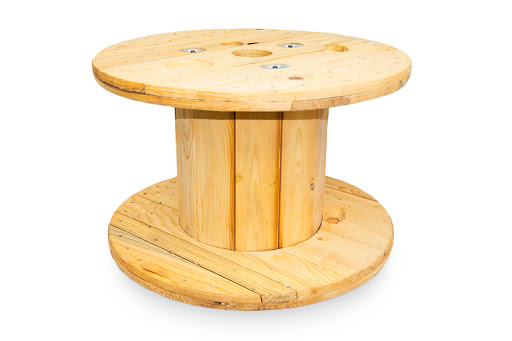
\includegraphics[width=0.8\textwidth]{image3}
	\caption{Bobina}
	\label{fig:mesh1}
\end{figure}



Da una bobina posso ricavare 2 tavoli. 
Ve ne sono di diverse misure, ho scelto quelle da 
$1200 mm$ e $1600 mm$, $H 1500 mm$.

\begin{figure}[H]
	\centering
	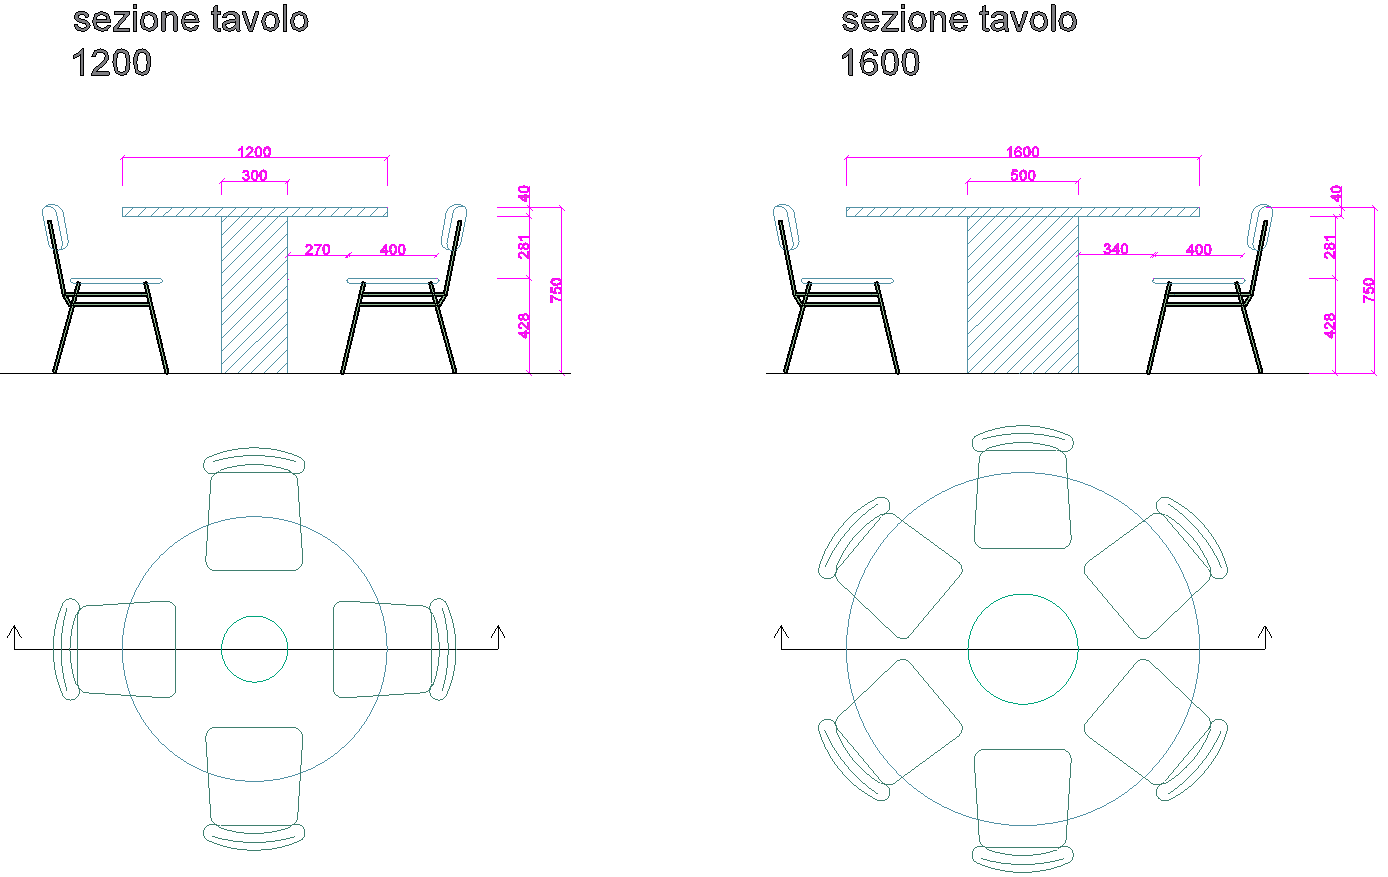
\includegraphics[width=0.8\textwidth]{image31}
	\caption{Sezione tavoli}
	\label{fig:mesh1}
\end{figure}

	\newpage
	\section{Conclusione}


In questa tesi è stato combinato il mio interesse per il lago di Endine e la passione per la progettazione . Mi è stata data l’occasione di  studiare, in modo approfondito, gli elementi che riguardano la realizzazione del bar; tema che non abbiamo potuto approfondire in classe. Al fine di creare un risultato interessante si è pensato di utilizzare  una struttura dal design non convenzionale, sul quale è stato adattato il progetto del bar. Il progetto è stato progettato interamente in CAD tutta la struttura è stata progettata tridimensionalmente al fine di poterla stampare in 3D. Infatti avere un oggetto tangibile alla fine della progettazione ci a permesso di valutare meglio la qualità della struttura ed individuare possibili difetti. Avere un prototipo in scala del progetto finale ci permette di mostrare al meglio il prodotto finale ad un possibile cliente.

Durante la formazione di apprendistato, della durata di 8 mesi, mi è stato permesso dall'azienda ospitante di utilizzare parte delle mie ore  nella progettazione; permettendomi  di imparare ad utilizzare un programma di disegno: Bsolid. Tutto questo mi ha maggiormente motivato a non terminare il mio percorso formativo e voler continuare con il quinto anno per ampliare maggiormente le mie competenze riguardanti il disegno. Tutto questo mi è necessario per poi poter accedere ad una formazione universitaria orientata al design. \\

\noindent
\cite{maggioli} ~ \cite{endine} ~ \cite{-_di_-_tecnica_here_2017} \cite{commercio} \cite{decreto}  \cite{design}
\cite{banconemis} \cite{bancone}  \cite{celle}
 \cite{caffe} \cite{decreto2} \cite{acqua} \cite{argine} \cite{documenti} \cite{barriere}



	\newpage
	\addcontentsline{toc}{section}{Sitografia}
	\printbibliography[heading=bibintoc, title={Sitografia}]	

	

\end{document}
